\documentclass[10pt,a4paper]{article}

% ---- Paladin | ACL-903 Milestone 1 | generated by scripts/build_report_latex.py ----
% Compile with pdfLaTeX (the Overleaf default). Every chart is drawn with pgfplots, so
% this one file is all you need: no images or data files to upload.

\usepackage[T1]{fontenc}
\usepackage[utf8]{inputenc}
\usepackage{mathptmx}
\usepackage[a4paper,left=17mm,right=17mm,top=20mm,bottom=19mm,headheight=19pt]{geometry}
\usepackage{microtype}
\usepackage[table,dvipsnames]{xcolor}
\usepackage{booktabs,array,colortbl}
\usepackage[font=small,labelfont=bf,labelsep=period,skip=4pt]{caption}
\usepackage{float}
\usepackage[section]{placeins}
\usepackage{titlesec}
\usepackage{fancyhdr}
\usepackage[most]{tcolorbox}
\usepackage{pgfplots}
\usepgfplotslibrary{groupplots}
\pgfplotsset{compat=1.17}
\usepackage[colorlinks=true,linkcolor=navy,urlcolor=navy,pdftitle={ACL-903 Milestone 1: Formula 1 podium prediction},pdfauthor={Paladin}]{hyperref}

\definecolor{navy}{HTML}{1E3A5F}
\definecolor{muted}{HTML}{5C6B7A}
\definecolor{zebra}{HTML}{F4F7FB}
\definecolor{modelA}{HTML}{4C72B0}
\definecolor{modelB}{HTML}{DD8452}
\definecolor{modelC}{HTML}{55A868}
\definecolor{splitA}{HTML}{264653}
\definecolor{splitB}{HTML}{F4A261}
\definecolor{splitC}{HTML}{E76F51}

\pgfplotsset{every axis/.append style={font=\footnotesize, tick label style={font=\scriptsize},
  label style={font=\scriptsize}, title style={font=\footnotesize\bfseries}, legend style={font=\scriptsize, draw=none, fill=none},
  /pgf/number format/1000 sep={}, /pgf/number format/fixed, scaled ticks=false}}

\setlength{\parindent}{0pt}
\setlength{\parskip}{4.2pt plus 1pt}
\renewcommand{\arraystretch}{1.12}
\setlength{\tabcolsep}{3.5pt}
\setlength{\textfloatsep}{10pt plus 2pt minus 2pt}
\setlength{\floatsep}{8pt plus 2pt minus 2pt}
\setlength{\intextsep}{8pt plus 2pt minus 2pt}

\titleformat{\section}{\large\bfseries\color{navy}}{\thesection.}{0.55em}{}
\titleformat{\subsection}{\normalsize\bfseries\color{navy!85!black}}{\thesubsection}{0.55em}{}
\titlespacing*{\section}{0pt}{12pt plus 3pt}{4pt}
\titlespacing*{\subsection}{0pt}{9pt plus 2pt}{3pt}

\pagestyle{fancy}
\fancyhf{}
\renewcommand{\headrulewidth}{0.5pt}
\renewcommand{\footrulewidth}{0.5pt}
\renewcommand{\headrule}{\hbox to\headwidth{\color{navy}\leaders\hrule height \headrulewidth\hfill}}
\renewcommand{\footrule}{\hbox to\headwidth{\color{navy}\leaders\hrule height \footrulewidth\hfill}}
\fancyhead[L]{\footnotesize\color{muted} ACL-903 Milestone 1}
\fancyhead[R]{\footnotesize\color{muted} Formula 1 podium prediction}
\fancyfoot[L]{\footnotesize\color{muted} Paladin}
\fancyfoot[R]{\footnotesize\color{muted} \thepage}

\newtcolorbox{takeaway}{enhanced, breakable, colback=zebra, colframe=navy, boxrule=0pt, leftrule=2.2pt,
  sharp corners, left=7pt, right=7pt, top=3pt, bottom=3pt, before skip=6pt, after skip=8pt}

\begin{document}
\sloppy
\thispagestyle{empty}
\vspace*{0.17\textheight}
\begin{center}
{\itshape\color{muted}\large ACL-903 Milestone 1\par}
\vspace{8pt}
{\fontsize{27}{31}\selectfont\bfseries\color{navy} Formula 1 podium prediction\par}
\vspace{8pt}
{\itshape\color{muted} An analytical report on leakage-safe prediction after qualifying\par}
\vspace{16pt}
{\color{navy}\rule{0.8\linewidth}{0.8pt}}\par
\vspace{16pt}
{\LARGE\bfseries\color{navy} Team Paladin\par}
\vspace{14pt}
{\small\setlength{\tabcolsep}{9pt}\renewcommand{\arraystretch}{1.35}
\begin{tabular}{llll}
\toprule
\textbf{Name} & \textbf{ID} & \textbf{Email} & \textbf{Tutorial} \\
\midrule
Ali Ussama Youssef & 58-2854 & ali.ussama@student.guc.edu.eg & T-25 \\
Yehia Wael Raafat Abdelfattah & 58-5798 & yehia.abdelfattah@student.guc.edu.eg & T-25 \\
Aya Ahmed Elkelany & 58-1764 & aya.elkelany@student.guc.edu.eg & T-14 \\
Rana Tamer Elsayed & 58-6459 &  & T-13 \\
\bottomrule
\end{tabular}}
\end{center}
\clearpage



\section{The question we are trying to answer}


In this report we ask a narrow question. After qualifying, and before the race starts, can we tell which drivers will finish in the top three? We use the Formula 1 World Championship tables from 1950 to 2024. The prediction cutoff matters. Anything that is only known once the race is underway, such as the finishing order, the points scored that day, the retirement reason, the pit stops, or the fastest lap, is not allowed into the model as an input for that same race.


The cleaned table has 26,668 driver-race rows, and 12.7\% of them are podiums. That rate is the reason we do not treat every metric as equal. A ranking that ignores the features would score a PR-AUC near 0.127 on the full table, and near 0.150 on the 2022-2024 seasons, because that is simply the share of positive rows. ROC-AUC answers a different question: if we pick one driver who podiumed and one who did not, how often does the model give the podium driver the higher probability? A coin-flip ranking sits near 0.500. We use PR-AUC as the main score and ROC-AUC as the secondary score. F1, precision, and recall are reported at one cutoff, and that cutoff is chosen only on 2020-2021.


\begin{takeaway}
\textbf{Takeaway.} The rest of the report follows that cutoff. First we check that the tables join cleanly and that the label is one row per driver per race. Then we answer three descriptive questions about front-row starts, home races, and mechanical retirements. Only after that do we train models, and we judge them by whether they rank the rare podium rows above the rest.
\end{takeaway}



\section{What we checked before trusting the joins}


The raw files are the 14 Kaggle/Ergast tables, and we do not edit them. The literal value \textbackslash{}N is read as missing. Dates are parsed as dates, and qualifying times such as 1:25.187 are converted to seconds. We then audited the keys that the later joins depend on.


Table 1 covers the eleven tables with a single-column primary key. Together they hold 100,621 rows. Every audited key is non-null, and none of these keys is duplicated. That is the check we needed before treating circuitId, driverId, raceId, and the other identifiers as safe join keys.


\begin{table}[H]
\centering
\caption{Primary-key audit of the raw tables. Null keys and duplicate keys are both zero in every audited table.}
{\small\rowcolors{2}{white}{zebra}
\begin{tabular}{>{\raggedright\arraybackslash}p{\dimexpr(\linewidth-10\tabcolsep)*246/1000\relax}>{\raggedright\arraybackslash}p{\dimexpr(\linewidth-10\tabcolsep)*270/1000\relax}>{\raggedleft\arraybackslash}p{\dimexpr(\linewidth-10\tabcolsep)*151/1000\relax}>{\raggedleft\arraybackslash}p{\dimexpr(\linewidth-10\tabcolsep)*151/1000\relax}>{\raggedleft\arraybackslash}p{\dimexpr(\linewidth-10\tabcolsep)*183/1000\relax}}
\toprule
\rowcolor{navy}
\textcolor{white}{\textbf{Table}} & \textcolor{white}{\textbf{Primary key}} & \textcolor{white}{\textbf{Rows}} & \textcolor{white}{\textbf{Null keys}} & \textcolor{white}{\textbf{Duplicate keys}} \\
\midrule
circuits & circuitId & 77 & 0 & 0 \\
constructors & constructorId & 212 & 0 & 0 \\
constructor\_results & constructorResultsId & 12,625 & 0 & 0 \\
constructor\_standings & constructorStandingsId & 13,391 & 0 & 0 \\
drivers & driverId & 861 & 0 & 0 \\
driver\_standings & driverStandingsId & 34,863 & 0 & 0 \\
races & raceId & 1,125 & 0 & 0 \\
results & resultId & 26,759 & 0 & 0 \\
qualifying & qualifyId & 10,494 & 0 & 0 \\
seasons & year & 75 & 0 & 0 \\
status & statusId & 139 & 0 & 0 \\
\bottomrule
\end{tabular}}
\end{table}


Table 2 checks the foreign keys we actually use. A result row should point at a real race, driver, constructor, and status. A race should point at a real circuit. Qualifying and both standings tables should point at real races. In every one of these relationships the orphan count is zero. The largest check is results.raceId, with 26,759 child rows and no missing parent.


\begin{table}[H]
\centering
\caption{Foreign-key audit. An orphan is a child value with no matching parent key. None were found.}
{\small\rowcolors{2}{white}{zebra}
\begin{tabular}{>{\raggedright\arraybackslash}p{\dimexpr(\linewidth-6\tabcolsep)*659/1000\relax}>{\raggedleft\arraybackslash}p{\dimexpr(\linewidth-6\tabcolsep)*198/1000\relax}>{\raggedleft\arraybackslash}p{\dimexpr(\linewidth-6\tabcolsep)*143/1000\relax}}
\toprule
\rowcolor{navy}
\textcolor{white}{\textbf{Relationship}} & \textcolor{white}{\textbf{Rows checked}} & \textcolor{white}{\textbf{Orphans}} \\
\midrule
races.circuitId $\rightarrow$ circuits.circuitId & 1,125 & 0 \\
results.raceId $\rightarrow$ races.raceId & 26,759 & 0 \\
results.driverId $\rightarrow$ drivers.driverId & 26,759 & 0 \\
results.constructorId $\rightarrow$ constructors.constructorId & 26,759 & 0 \\
results.statusId $\rightarrow$ status.statusId & 26,759 & 0 \\
qualifying.raceId $\rightarrow$ races.raceId & 10,494 & 0 \\
qualifying.driverId $\rightarrow$ drivers.driverId & 10,494 & 0 \\
driver\_standings.raceId $\rightarrow$ races.raceId & 34,863 & 0 \\
constructor\_standings.raceId $\rightarrow$ races.raceId & 13,391 & 0 \\
\bottomrule
\end{tabular}}
\end{table}


The results file has 26,759 rows, but it is not yet one row per driver per race. Early shared drives produce more than one result for the same driver in the same race. We found 85 such driver-race groups. The rule we keep is deterministic: prefer the row with a real grid start (grid greater than 0), then the better finishing position, then the smaller resultId. After that rule, 26,668 rows remain, each pair (raceId, driverId) appears once, and the seasons run from 1950 to 2024.


Grid position 0 is not a better starting spot than pole. In this table it accounts for 6.1\% of rows. We keep it as a pit-lane flag and treat the numeric grid position as missing in those rows, so the model cannot learn that 0 is the front of the field.


\begin{figure}[H]
\centering
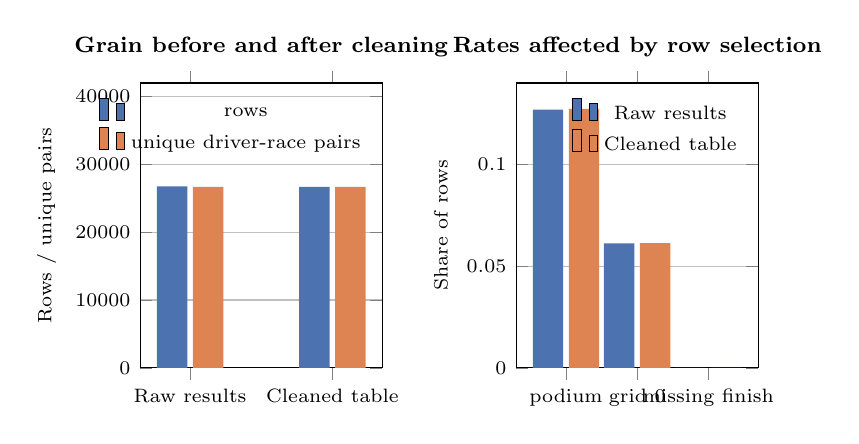
\begin{tikzpicture}
\begin{groupplot}[group style={group size=2 by 1, horizontal sep=1.7cm}, width=0.384\linewidth, height=5.2cm, ymajorgrids, enlarge x limits=0.35]
\nextgroupplot[ybar, bar width=11pt, title={Grain before and after cleaning}, ylabel={Rows / unique pairs}, xtick={0,1}, xticklabels={Raw results,Cleaned table}, ymin=0, ymax=42000, scaled y ticks=false, legend pos=north east]
\addplot[fill=modelA, draw=none] coordinates {(0,26759) (1,26668)};
\addplot[fill=modelB, draw=none] coordinates {(0,26668) (1,26668)};
\legend{rows, unique driver-race pairs}
\nextgroupplot[ybar, bar width=11pt, title={Rates affected by row selection}, ylabel={Share of rows}, xtick={0,1,2}, xticklabels={podium,grid 0,missing finish}, ymin=0, legend pos=north east]
\addplot[fill=modelA, draw=none] coordinates {(0,0.126948) (1,0.061213) (2,0)};
\addplot[fill=modelB, draw=none] coordinates {(0,0.127306) (1,0.0613094) (2,0)};
\legend{Raw results, Cleaned table}
\end{groupplot}
\end{tikzpicture}
\caption{Programmatic EDA before and after duplicate cleaning. The left panel compares total rows with unique driver-race pairs; the right panel checks whether row selection materially changes key rates.}
\end{figure}


\begin{table}[H]
\centering
\caption{Before-and-after cleaning diagnostics computed from the raw results and cleaned modeling table.}
{\footnotesize\rowcolors{2}{white}{zebra}
\begin{tabular}{>{\raggedright\arraybackslash}p{\dimexpr(\linewidth-16\tabcolsep)*201/1000\relax}>{\raggedleft\arraybackslash}p{\dimexpr(\linewidth-16\tabcolsep)*100/1000\relax}>{\raggedleft\arraybackslash}p{\dimexpr(\linewidth-16\tabcolsep)*126/1000\relax}>{\raggedleft\arraybackslash}p{\dimexpr(\linewidth-16\tabcolsep)*132/1000\relax}>{\raggedleft\arraybackslash}p{\dimexpr(\linewidth-16\tabcolsep)*100/1000\relax}>{\raggedleft\arraybackslash}p{\dimexpr(\linewidth-16\tabcolsep)*93/1000\relax}>{\raggedleft\arraybackslash}p{\dimexpr(\linewidth-16\tabcolsep)*132/1000\relax}>{\raggedleft\arraybackslash}p{\dimexpr(\linewidth-16\tabcolsep)*116/1000\relax}}
\toprule
\rowcolor{navy}
\textcolor{white}{\textbf{Stage}} & \textcolor{white}{\textbf{Rows}} & \textcolor{white}{\textbf{Unique pairs}} & \textcolor{white}{\textbf{Duplicate rows}} & \textcolor{white}{\textbf{Podiums}} & \textcolor{white}{\textbf{Grid 0}} & \textcolor{white}{\textbf{Missing finish}} & \textcolor{white}{\textbf{Median grid}} \\
\midrule
Raw results & 26,759 & 26,668 & 176 & 12.7\% & 6.1\% & 0.0\% & 12.0 \\
Cleaned modeling table & 26,668 & 26,668 & 0 & 12.7\% & 6.1\% & 0.0\% & 12.0 \\
\bottomrule
\end{tabular}}
\end{table}


In cleaning we remove 91 extra shared-drive rows. Duplicate participation falls from 176 rows to zero, while the podium rate moves only from 12.7\% to 12.7\% and the median non-zero grid remains 12.0. So we fix the prediction grain without materially reshaping the label or the starting-position distribution.


\begin{takeaway}
\textbf{Takeaway.} The joins we rely on later are supported by the key audit, and the modelling grain is one driver in one race. The cleaning choices are recorded so that a shared drive cannot silently become two training rows.
\end{takeaway}



\section{Qualifying coverage is not stable across history}


Qualifying position is an obvious pre-race feature, but it is not recorded for most of the early championship. Figure 2 plots, for each season, the share of driver-race rows that have a qualifying position. We use this plot to decide whether we can drop seasons that lack qualifying, or whether we have to keep a feature that survives the whole time span.


\begin{figure}[H]
\centering
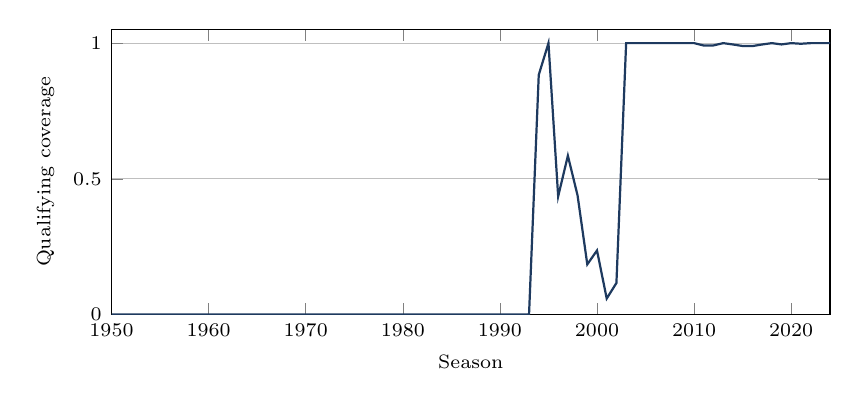
\begin{tikzpicture}
\begin{axis}[width=0.883\linewidth, height=5.2cm, xlabel={Season}, ylabel={Qualifying coverage}, ymin=0, ymax=1.05, xmin=1950, xmax=2024, ymajorgrids, scaled ticks=false, xtick distance=10]
\addplot[navy, thick] coordinates {(1950,0) (1951,0) (1952,0) (1953,0) (1954,0) (1955,0) (1956,0) (1957,0) (1958,0) (1959,0) (1960,0) (1961,0) (1962,0) (1963,0) (1964,0) (1965,0) (1966,0) (1967,0) (1968,0) (1969,0) (1970,0) (1971,0) (1972,0) (1973,0) (1974,0) (1975,0) (1976,0) (1977,0) (1978,0) (1979,0) (1980,0) (1981,0) (1982,0) (1983,0) (1984,0) (1985,0) (1986,0) (1987,0) (1988,0) (1989,0) (1990,0) (1991,0) (1992,0) (1993,0) (1994,0.882883) (1995,1) (1996,0.435294) (1997,0.585106) (1998,0.438395) (1999,0.184659) (2000,0.235925) (2001,0.0588235) (2002,0.116022) (2003,1) (2004,1) (2005,1) (2006,1) (2007,1) (2008,1) (2009,1) (2010,1) (2011,0.991228) (2012,0.991667) (2013,1) (2014,0.995086) (2015,0.989418) (2016,0.989177) (2017,0.995) (2018,1) (2019,0.995238) (2020,1) (2021,0.997727) (2022,1) (2023,1) (2024,1)};
\end{axis}
\end{tikzpicture}
\caption{Share of driver-race rows with a recorded qualifying position, by season. Coverage is essentially zero until the mid-1990s, unstable until 2003, and then close to complete.}
\end{figure}


In our modelling table, coverage is 0\% in 1950 and still 0\% in 1993. It jumps to 88.3\% in 1994 and 100\% in 1995, then falls again. The low point of that second gap is 5.9\% in 2001. From 2003 onwards the line sits on or next to 100\%, and 2024 is 100\%. Averaged over seasons, coverage is 7.1\% before 2000 and 89.4\% from 2000 on. At row level, 60.6\% of all driver-races have no qualifying position.


We observe two different regimes, not a smooth rise. The early championship has almost no qualifying rows in this snapshot. The seasons from 1994 to 2002 are patchy. The seasons we later use for validation and test are essentially complete. Dropping the early years would throw away most of the history, and it would also make the training set look more like the test set than it really is. We keep every season, store an explicit missingness flag, and treat grid position as the starting-order feature that exists throughout. The flag lets the model see that a qualifying value was absent, rather than hiding that fact inside a filled-in number.


\begin{takeaway}
\textbf{Takeaway.} Qualifying is a modern-era measurement in this dataset. Any model that depends on it alone would be fitting 2003-2024 and guessing before that. Grid position is the feature that can be compared across the whole 75 seasons.
\end{takeaway}



\section{Three questions about the races, before any model}


The prediction model comes later. These three questions use the joined tables directly. We separate what the counts show from what we are willing to infer. None of the three answers is a causal claim.



\subsection{Front-row starts convert to podiums much more often than other starts}


A front-row start means grid position 1 or 2 on the final grid. We do not use qualifying position for this definition. A penalty can move a driver back between qualifying and the start, and the car that lines up first is the one we want. Results are joined to races and then to circuits. We split the history at 2014, the hybrid-era change, and we only rank a circuit inside an era when it has at least ten front-row starts there. That filter leaves 44 circuits in 1950-2013 and 19 circuits in 2014-2024.


\begin{figure}[H]
\centering
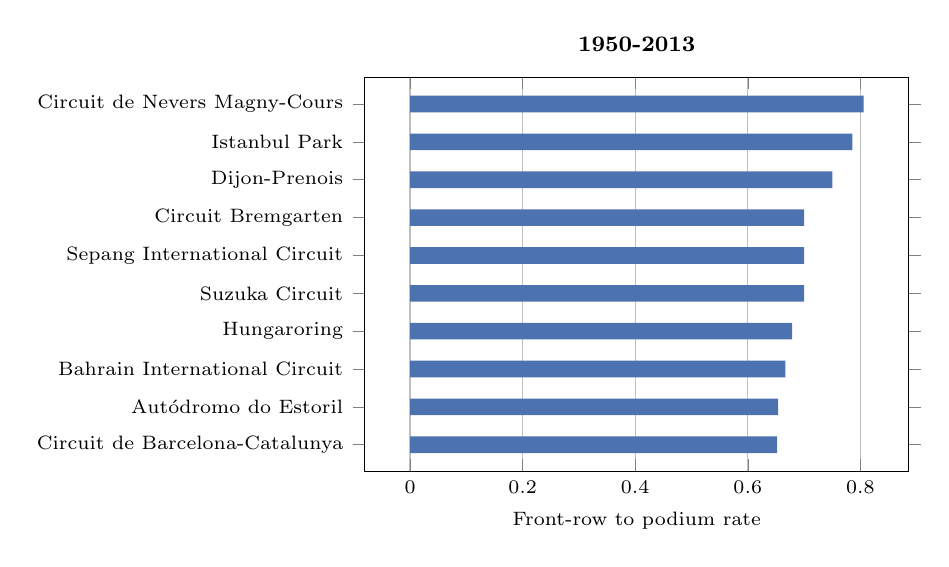
\begin{tikzpicture}
\begin{axis}[xbar, bar width=6pt, width=0.570\linewidth, height=5.0cm, scale only axis, ytick={0,1,2,3,4,5,6,7,8,9}, yticklabels={Circuit de Nevers Magny-Cours,Istanbul Park,Dijon-Prenois,Circuit Bremgarten,Sepang International Circuit,Suzuka Circuit,Hungaroring,Bahrain International Circuit,Autódromo do Estoril,Circuit de Barcelona-Catalunya}, y dir=reverse, ymin=-0.7, ymax=9.7, xlabel={Front-row to podium rate}, xmajorgrids, xmin=0, yticklabel style={font=\scriptsize}, enlarge x limits=0.1, title={1950-2013}, ]
\addplot[xbar, fill=modelA, draw=none] coordinates {(0.805556,0) (0.785714,1) (0.75,2) (0.7,3) (0.7,4) (0.7,5) (0.678571,6) (0.666667,7) (0.653846,8) (0.652174,9)};
\end{axis}
\end{tikzpicture}
\medskip
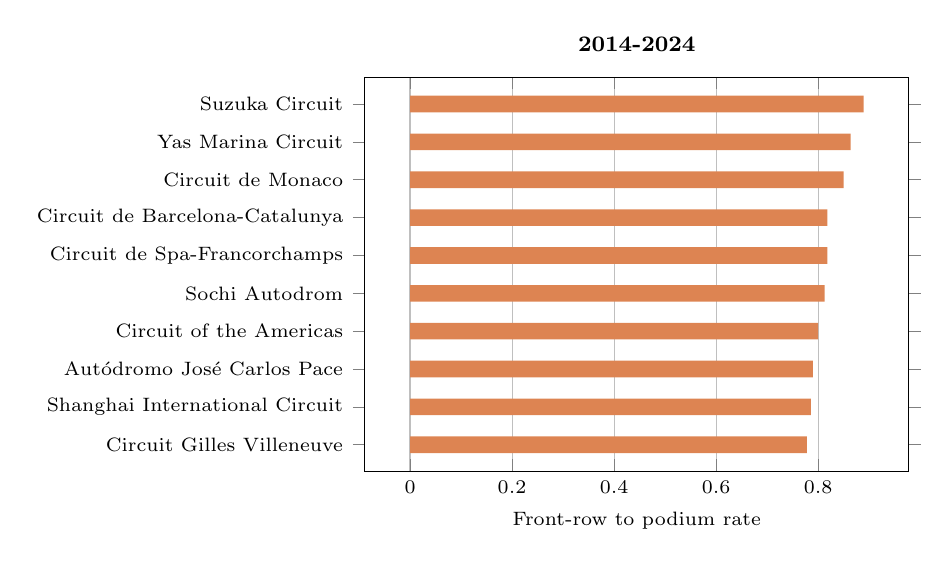
\begin{tikzpicture}
\begin{axis}[xbar, bar width=6pt, width=0.570\linewidth, height=5.0cm, scale only axis, ytick={0,1,2,3,4,5,6,7,8,9}, yticklabels={Suzuka Circuit,Yas Marina Circuit,Circuit de Monaco,Circuit de Barcelona-Catalunya,Circuit de Spa-Francorchamps,Sochi Autodrom,Circuit of the Americas,Autódromo José Carlos Pace,Shanghai International Circuit,Circuit Gilles Villeneuve}, y dir=reverse, ymin=-0.7, ymax=9.7, xlabel={Front-row to podium rate}, xmajorgrids, xmin=0, yticklabel style={font=\scriptsize}, enlarge x limits=0.1, title={2014-2024}, ]
\addplot[xbar, fill=modelB, draw=none] coordinates {(0.888889,0) (0.863636,1) (0.85,2) (0.818182,3) (0.818182,4) (0.8125,5) (0.8,6) (0.789474,7) (0.785714,8) (0.777778,9)};
\end{axis}
\end{tikzpicture}
\caption{Ten circuits with the highest front-row podium rate in each era. The rate is podiums divided by front-row starts. Circuits with fewer than ten such starts are excluded.}
\end{figure}


\begin{table}[H]
\centering
\caption{Highest front-row podium rates in each era, among circuits with at least ten front-row starts. The rate is a proportion of starts, not a mean of lap times.}
{\small\rowcolors{2}{white}{zebra}
\begin{tabular}{>{\raggedright\arraybackslash}p{\dimexpr(\linewidth-8\tabcolsep)*168/1000\relax}>{\raggedright\arraybackslash}p{\dimexpr(\linewidth-8\tabcolsep)*460/1000\relax}>{\raggedleft\arraybackslash}p{\dimexpr(\linewidth-8\tabcolsep)*168/1000\relax}>{\raggedleft\arraybackslash}p{\dimexpr(\linewidth-8\tabcolsep)*204/1000\relax}}
\toprule
\rowcolor{navy}
\textcolor{white}{\textbf{Era}} & \textcolor{white}{\textbf{Circuit}} & \textcolor{white}{\textbf{Podium rate}} & \textcolor{white}{\textbf{Front-row starts}} \\
\midrule
1950-2013 & Circuit de Nevers Magny-Cours & 80.6\% & 36 \\
1950-2013 & Istanbul Park & 78.6\% & 14 \\
1950-2013 & Dijon-Prenois & 75.0\% & 12 \\
1950-2013 & Circuit Bremgarten & 70.0\% & 10 \\
1950-2013 & Sepang International Circuit & 70.0\% & 30 \\
2014-2024 & Suzuka Circuit & 88.9\% & 18 \\
2014-2024 & Yas Marina Circuit & 86.4\% & 22 \\
2014-2024 & Circuit de Monaco & 85.0\% & 20 \\
2014-2024 & Circuit de Barcelona-Catalunya & 81.8\% & 22 \\
2014-2024 & Circuit de Spa-Francorchamps & 81.8\% & 22 \\
\bottomrule
\end{tabular}}
\end{table}


What we see is a shift in level, not just a change of leader. Across circuits that pass the ten-start rule, the median front-row podium rate is 56.8\% in 1950-2013 and 77.8\% in 2014-2024. The early range runs from 28.6\% at Detroit Street Circuit (14 starts) up to 80.6\% at Magny-Cours (36 starts). The modern range runs from 59.1\% at Hungaroring (22 starts) up to 88.9\% at Suzuka (18 starts).


If we ignore the circuit filter and use every front-row start in the modelling table, the rate is 56.0\% of 1,789 starts before 2014, and 76.0\% of 454 starts from 2014 on. The podium rate among all starters, not just the front row, is 12.3\% and 14.8\% in those same eras. A front-row car is therefore several times more likely to podium than a typical starter. The modern front row converts at a higher rate than the historical front row, while the all-starter rate only moves from about 12\% to about 15\%.


The ranking itself needs a sample-size caution. Istanbul Park is second in the early list at 78.6\%, but that is 14 starts. Dijon-Prenois and Bremgarten sit near the top with 12 and 10 starts. Magny-Cours (36 starts) and Sepang (30 starts) are firmer early observations. The next early circuit, Suzuka, is also at 70\%, and it has 50 starts, so that rate is not carried only by Bremgarten. In 2014-2024 the leading circuits each have between 18 and 22 starts, so the order is less sensitive to one or two races, but Suzuka's 88.9\% is still 18 starts, not a long census. We can say the leaders change with the era. We cannot say that a circuit causes the conversion rate. The front row is already occupied by the fastest cars.


\begin{takeaway}
\textbf{Takeaway.} Where a driver starts dominates this descriptive cut. Era changes the level of front-row conversion, and the circuit ranking is real under our ten-start rule, with wide uncertainty on the circuits that barely meet it.
\end{takeaway}



\subsection{Once the grid band is fixed, home drivers do not podium more often}


The second question is whether drivers do better at a home race. We map nationality to a circuit country (British to the UK, Dutch to the Netherlands, and so on) and mark a row as home when those match. Drivers whose nationality is not in the map are left out. We then compare home and away podium rates inside the same grid bands, because Section 4.1 already shows that starting position can overwhelm a smaller effect. Figure 4 plots the two series.


\begin{figure}[H]
\centering
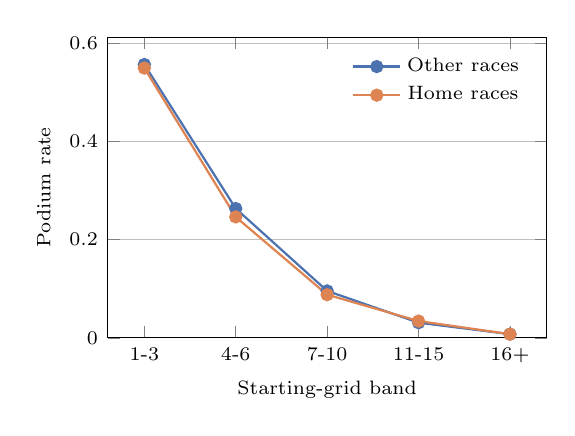
\begin{tikzpicture}
\begin{axis}[width=0.590\linewidth, height=5.4cm, xlabel={Starting-grid band}, ylabel={Podium rate}, xtick={0,1,2,3,4}, xticklabels={1-3,4-6,7-10,11-15,16+}, ymin=0, ymajorgrids, legend pos=north east, enlarge x limits=0.1]
\addplot[modelA, thick, mark=*] coordinates {(0,0.556536) (1,0.263263) (2,0.0954887) (3,0.0308129) (4,0.00753187)};
\addplot[modelB, thick, mark=*] coordinates {(0,0.549242) (1,0.246154) (2,0.0878553) (3,0.0341151) (4,0.00747863)};
\legend{Other races, Home races}
\end{axis}
\end{tikzpicture}
\caption{Podium rate by starting-grid band for home races (home\_race = True) and other races (home\_race = False). The two lines fall together as the start position gets worse.}
\end{figure}


\begin{table}[H]
\centering
\caption{Podium rate by grid band and home status. The last column is the home rate minus the away rate, in percentage points.}
{\small\rowcolors{2}{white}{zebra}
\begin{tabular}{>{\raggedright\arraybackslash}p{\dimexpr(\linewidth-12\tabcolsep)*148/1000\relax}>{\raggedleft\arraybackslash}p{\dimexpr(\linewidth-12\tabcolsep)*148/1000\relax}>{\raggedleft\arraybackslash}p{\dimexpr(\linewidth-12\tabcolsep)*165/1000\relax}>{\raggedleft\arraybackslash}p{\dimexpr(\linewidth-12\tabcolsep)*157/1000\relax}>{\raggedleft\arraybackslash}p{\dimexpr(\linewidth-12\tabcolsep)*165/1000\relax}>{\raggedleft\arraybackslash}p{\dimexpr(\linewidth-12\tabcolsep)*217/1000\relax}}
\toprule
\rowcolor{navy}
\textcolor{white}{\textbf{Grid band}} & \textcolor{white}{\textbf{Away rate}} & \textcolor{white}{\textbf{Away starts}} & \textcolor{white}{\textbf{Home rate}} & \textcolor{white}{\textbf{Home starts}} & \textcolor{white}{\textbf{Home minus away}} \\
\midrule
1-3 & 55.7\% & 3,060 & 54.9\% & 264 & $-$0.7 pp \\
4-6 & 26.3\% & 3,016 & 24.6\% & 260 & $-$1.7 pp \\
7-10 & 9.5\% & 3,990 & 8.8\% & 387 & $-$0.8 pp \\
11-15 & 3.1\% & 4,933 & 3.4\% & 469 & +0.3 pp \\
16+ & 0.8\% & 6,904 & 0.7\% & 936 & $-$0.0 pp \\
\bottomrule
\end{tabular}}
\end{table}


What we find in Figure 4 and Table 5 is the grid, not the passport. Away drivers podium 55.7\% of the time from positions 1-3 (3,060 starts), 26.3\% from 4-6, 9.5\% from 7-10, 3.1\% from 11-15, and 0.8\% from 16th or worse. Home drivers track those rates: 54.9\%, 24.6\%, 8.8\%, 3.4\%, and 0.7\%.


The home-minus-away gaps we measure are $-$0.7, $-$1.7, $-$0.8, +0.3, and $-$0.0 percentage points. Four of the five bands are slightly negative. The only positive gap is positions 11-15, and it is +0.3 percentage points.


Home samples are also much smaller. In the front band we have 264 home starts against 3,060 away starts, so a gap under one percentage point is not a stable difference. Compared with the drop from the front band (about 55\%) to the back band (under 1\%), the home contrast is small.


This suggests that a raw home-versus-away average would mostly pick up who starts near the front, not a separate home advantage. The stratification is a control, not a causal model. The nationality map also misses drivers we could not assign, and it cannot represent dual nationality. We therefore report a descriptive result: inside a grid band, home drivers in this table do not show a consistent podium advantage.


\begin{takeaway}
\textbf{Takeaway.} Starting position sorts podium rates into a steep ladder. Home status, measured this way, does not move a driver from one rung to another.
\end{takeaway}



\subsection{Mechanical retirement rates are lower in 2022-2024, and small teams sit at the top of each list}


The third question is which constructors retire with a mechanical failure, and whether that rate changed between 2014-2021 and 2022-2024. We join results to status and constructor. A start counts as mechanical only when the status text is on a fixed list of component failures: engine, gearbox, brakes, hydraulics, power unit, and the other documented part failures. Crashes, driver errors, disqualifications, and collisions are not on that list. Cars that did not start are removed from the denominator. Those statuses are Did not prequalify, Did not qualify, Did not start, Excluded, Withdrew. A constructor-era needs at least 20 starts to appear. The rate is mechanical retirements divided by starts, so a team that finishes races is in the denominator even when it rarely fails.


{\small The included statuses are: Alternator, Battery, Brake duct, Brakes, Clutch, Cooling system, Differential, Driveshaft, Drivetrain, ERS, Electrical, Electronics, Engine, Exhaust, Fire, Front wing, Fuel leak, Fuel pressure, Fuel pump, Fuel system, Gearbox, Hydraulics, Mechanical, Oil leak, Oil pressure, Overheating, Power Unit, Power loss, Puncture, Radiator, Rear wing, Safety belt, Spark plugs, Steering, Suspension, Technical, Throttle, Transmission, Turbo, Tyre, Tyre puncture, Undertray, Vibrations, Water leak, Water pressure, Water pump, Wheel, Wheel bearing, Wheel nut. Rare wordings that are not on this list are counted as non-mechanical. That choice can miss an ambiguous failure, and it can also avoid treating a collision as a broken part. We would rather under-count borderline cases than inflate the rate.\par}


\begin{figure}[H]
\centering
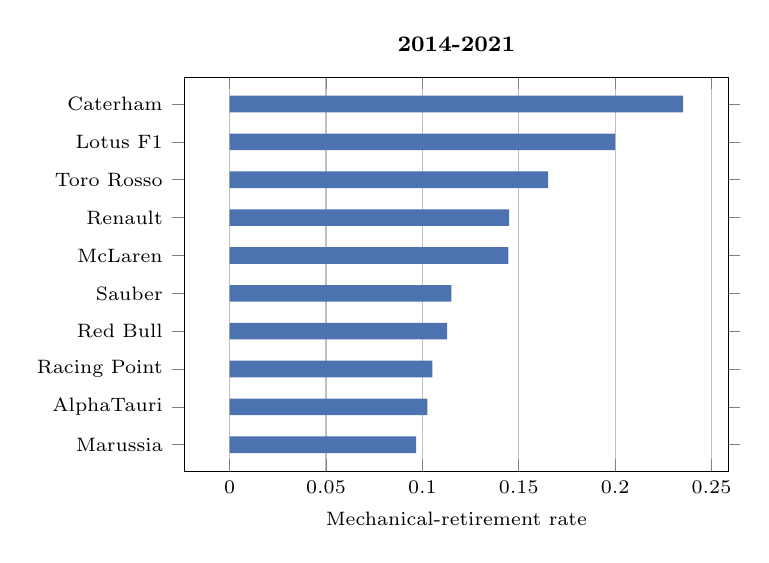
\begin{tikzpicture}
\begin{axis}[xbar, bar width=6pt, width=0.570\linewidth, height=5.0cm, scale only axis, ytick={0,1,2,3,4,5,6,7,8,9}, yticklabels={Caterham,Lotus F1,Toro Rosso,Renault,McLaren,Sauber,Red Bull,Racing Point,AlphaTauri,Marussia}, y dir=reverse, ymin=-0.7, ymax=9.7, xlabel={Mechanical-retirement rate}, xmajorgrids, xmin=0, yticklabel style={font=\scriptsize}, enlarge x limits=0.1, title={2014-2021}, ]
\addplot[xbar, fill=modelA, draw=none] coordinates {(0.235294,0) (0.2,1) (0.165289,2) (0.145,3) (0.144654,4) (0.115,5) (0.112853,6) (0.105263,7) (0.102564,8) (0.0967742,9)};
\end{axis}
\end{tikzpicture}
\medskip
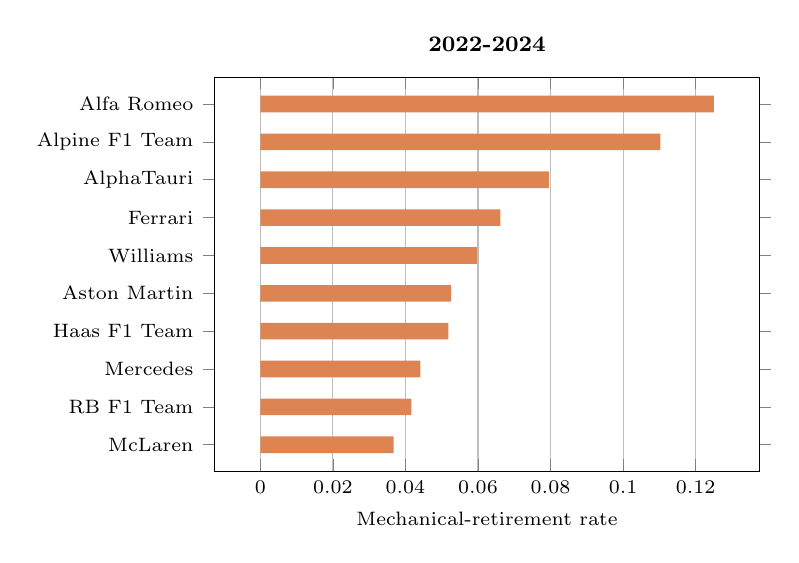
\begin{tikzpicture}
\begin{axis}[xbar, bar width=6pt, width=0.570\linewidth, height=5.0cm, scale only axis, ytick={0,1,2,3,4,5,6,7,8,9}, yticklabels={Alfa Romeo,Alpine F1 Team,AlphaTauri,Ferrari,Williams,Aston Martin,Haas F1 Team,Mercedes,RB F1 Team,McLaren}, y dir=reverse, ymin=-0.7, ymax=9.7, xlabel={Mechanical-retirement rate}, xmajorgrids, xmin=0, yticklabel style={font=\scriptsize}, enlarge x limits=0.1, title={2022-2024}, ]
\addplot[xbar, fill=modelB, draw=none] coordinates {(0.125,0) (0.110294,1) (0.0795455,2) (0.0661765,3) (0.0597015,4) (0.0526316,5) (0.0518519,6) (0.0441176,7) (0.0416667,8) (0.0367647,9)};
\end{axis}
\end{tikzpicture}
\caption{Ten constructors with the highest mechanical-retirement rate in each era, among those with at least 20 starts. The rate uses all starts as the denominator.}
\end{figure}


Among constructors that meet the 20-start rule, we count 329 mechanical retirements in 3,257 starts in 2014-2021 (10.1\%), and 83 mechanical retirements in 1,354 starts in 2022-2024 (6.1\%). The median constructor rate falls from 9.7\% to 5.2\%. That is 19 constructors in the first era and 12 in the second. Figure 5 shows the high end of each list. Table 6 also shows the low end, because a chart of only the worst rates makes an era look less reliable than it is.


\begin{table}[H]
\centering
\caption{Highest and lowest mechanical-retirement rates in each era, plus a few large teams for scale. Rate = failures / starts, after removing non-starts.}
{\small\rowcolors{2}{white}{zebra}
\begin{tabular}{>{\raggedright\arraybackslash}p{\dimexpr(\linewidth-10\tabcolsep)*207/1000\relax}>{\raggedright\arraybackslash}p{\dimexpr(\linewidth-10\tabcolsep)*306/1000\relax}>{\raggedleft\arraybackslash}p{\dimexpr(\linewidth-10\tabcolsep)*153/1000\relax}>{\raggedleft\arraybackslash}p{\dimexpr(\linewidth-10\tabcolsep)*171/1000\relax}>{\raggedleft\arraybackslash}p{\dimexpr(\linewidth-10\tabcolsep)*162/1000\relax}}
\toprule
\rowcolor{navy}
\textcolor{white}{\textbf{Era}} & \textcolor{white}{\textbf{Constructor}} & \textcolor{white}{\textbf{Rate}} & \textcolor{white}{\textbf{Failures}} & \textcolor{white}{\textbf{Starts}} \\
\midrule
2014-2021 & Caterham & 23.5\% & 8 & 34 \\
2014-2021 & Lotus F1 & 20.0\% & 15 & 75 \\
2014-2021 & Toro Rosso & 16.5\% & 40 & 242 \\
2014-2021 & Mercedes & 4.4\% & 14 & 320 \\
2014-2021 & Aston Martin & 2.3\% & 1 & 44 \\
2022-2024 & Alfa Romeo & 12.5\% & 11 & 88 \\
2022-2024 & Alpine F1 Team & 11.0\% & 15 & 136 \\
2022-2024 & AlphaTauri & 8.0\% & 7 & 88 \\
2022-2024 & Red Bull & 3.7\% & 5 & 136 \\
2022-2024 & McLaren & 3.7\% & 5 & 136 \\
2022-2024 & Sauber & 2.1\% & 1 & 48 \\
\bottomrule
\end{tabular}}
\end{table}


In our table Caterham has the highest 2014-2021 rate, 23.5\%, which is 8 failures in 34 starts. Mercedes, over 320 starts, sits at 4.4\% (14 failures). Aston Martin's 2.3\% is 1 failure in 44 starts, so the bottom of that list is also a small sample. In 2022-2024, Alfa Romeo leads at 12.5\% (11 of 88), while Sauber is at 2.1\% (1 of 48). Red Bull and McLaren are both at 3.7\% on 136 starts.


An interesting observation is the Alfa Romeo name across the cut: 4.2\% in 2014-2021 (5 of 120 starts) against 12.5\% in 2022-2024. The same constructor name does not mean the same car, and this table does not say why the rate rose. What the table does show is that the top of each era is a smaller or shorter-lived entry, while the large teams are clustered well below the leaders. The era totals are lower after 2021. One reading is the 2022 regulation change. The status strings and the 20-start filter can also move the rate, so we stop at the comparison.


\begin{takeaway}
\textbf{Takeaway.} Mechanical retirements, under this definition, are less common in 2022-2024 than in 2014-2021. The identity of the highest-rate constructor changes, and those leading rates rest on fewer starts than the works teams.
\end{takeaway}



\section{What the model is allowed to see}


The descriptive results above already point at the grid. The modelling step has to respect the cutoff. We build 17 inputs in five groups. Form uses a shift before the rolling window, so today's result is not inside today's features. Constructor form is averaged across both cars first, so one teammate cannot see the other teammate's result from the same race. Championship points and rank are taken from the previous race in the same season, because a standings row describes the table after a race. The first race of a season, and a driver's first race, therefore have missing history, and we leave those values missing rather than filling them with the future.


\begin{table}[H]
\centering
\caption{Feature groups. Post-race position, points scored today, laps, status, pit stops, and fastest lap are excluded.}
{\small\rowcolors{2}{white}{zebra}
\begin{tabular}{>{\raggedright\arraybackslash}p{\dimexpr(\linewidth-6\tabcolsep)*168/1000\relax}>{\raggedright\arraybackslash}p{\dimexpr(\linewidth-6\tabcolsep)*460/1000\relax}>{\raggedright\arraybackslash}p{\dimexpr(\linewidth-6\tabcolsep)*372/1000\relax}}
\toprule
\rowcolor{navy}
\textcolor{white}{\textbf{Group}} & \textcolor{white}{\textbf{Inputs}} & \textcolor{white}{\textbf{Why it is known before the start}} \\
\midrule
Grid & Grid position, pit-lane flag, front-row flag, field size & Final grid is set before lights out \\
Qualifying & Position, best Q1/Q2/Q3 time, missingness flag & Qualifying is already finished \\
Form & Driver and constructor podium rate over the previous 5 races, prior starts & Current race is shifted out \\
Standings & Driver and constructor points and rank & Attached from the previous race only \\
Context & Driver age, championship round, year & Known on race morning \\
\bottomrule
\end{tabular}}
\end{table}


We split by season, not at random. A random split would let 2023 teach the model about 2022. Training is every season through 2019, validation is 2020-2021, and the test seasons 2022-2024 are scored once. Training fits the imputer, scaler, and weights; validation makes every choice (preprocessing, ablation, model, cutoff); test is only reported. Table 8 shows why that split is not a copy of the same problem three times.


\begin{table}[H]
\centering
\caption{Time split used for every model. Starters per race is the number of modelling rows divided by races.}
{\footnotesize\rowcolors{2}{white}{zebra}
\begin{tabular}{>{\raggedright\arraybackslash}p{\dimexpr(\linewidth-14\tabcolsep)*147/1000\relax}>{\raggedright\arraybackslash}p{\dimexpr(\linewidth-14\tabcolsep)*147/1000\relax}>{\raggedleft\arraybackslash}p{\dimexpr(\linewidth-14\tabcolsep)*116/1000\relax}>{\raggedleft\arraybackslash}p{\dimexpr(\linewidth-14\tabcolsep)*101/1000\relax}>{\raggedleft\arraybackslash}p{\dimexpr(\linewidth-14\tabcolsep)*163/1000\relax}>{\raggedleft\arraybackslash}p{\dimexpr(\linewidth-14\tabcolsep)*140/1000\relax}>{\raggedleft\arraybackslash}p{\dimexpr(\linewidth-14\tabcolsep)*186/1000\relax}}
\toprule
\rowcolor{navy}
\textcolor{white}{\textbf{Split}} & \textcolor{white}{\textbf{Seasons}} & \textcolor{white}{\textbf{Rows}} & \textcolor{white}{\textbf{Races}} & \textcolor{white}{\textbf{Starters / race}} & \textcolor{white}{\textbf{Podium rate}} & \textcolor{white}{\textbf{Qualifying missing}} \\
\midrule
Training & 1950-2019 & 24,529 & 1,018 & 24.1 & 12.5\% & 65.9\% \\
Validation & 2020-2021 & 780 & 39 & 20.0 & 15.0\% & 0.1\% \\
Test & 2022-2024 & 1,359 & 68 & 20.0 & 15.0\% & 0.0\% \\
\bottomrule
\end{tabular}}
\end{table}


Our training seasons have 24,529 rows and 1,018 races, but 65.9\% of those rows have no qualifying result. Validation has only 780 rows and 39 races, and the test set has 1,359 rows and 68 races. Qualifying is almost complete in both recent splits (0.1\% missing in validation, 0\% in test). The podium rate rises from 12.5\% in training to 15.0\% and 15.0\% later. That matches the field size: training averages 24.1 starters per race, against 20.0 in validation. There are still three podium places, shared across fewer cars.


All 7 of our split checks pass: every row is assigned once, no race appears in two splits, and the last training race is before the first validation race, which is before the first test race. Figure 6 shows the split on the season axis together with the two quantities that drift across it.


\begin{figure}[H]
\centering
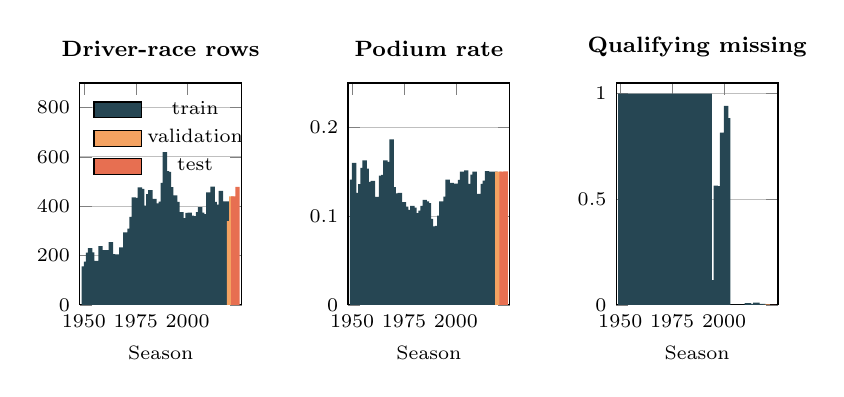
\begin{tikzpicture}
\begin{groupplot}[group style={group size=3 by 1, horizontal sep=1.35cm}, width=0.300\linewidth, height=4.4cm, ymajorgrids, xmin=1948, xmax=2026]
\nextgroupplot[title={Driver-race rows}, xlabel={Season}, ymin=0, ymax=900, xtick={1950,1975,2000}, scaled ticks=false, area legend, legend pos=north west]
\addplot[ybar, bar shift=0pt, bar width=1.6pt, fill=splitA, draw=none] coordinates {(1950,156) (1951,175) (1952,212) (1953,230) (1954,213) (1955,162) (1956,178) (1957,163) (1958,238) (1959,195) (1960,222) (1961,218) (1962,222) (1963,254) (1964,206) (1965,205) (1966,166) (1967,205) (1968,233) (1969,177) (1970,294) (1971,263) (1972,309) (1973,357) (1974,436) (1975,363) (1976,434) (1977,477) (1978,470) (1979,403) (1980,383) (1981,449) (1982,465) (1983,424) (1984,430) (1985,406) (1986,412) (1987,419) (1988,495) (1989,620) (1990,542) (1991,539) (1992,478) (1993,412) (1994,444) (1995,418) (1996,340) (1997,376) (1998,349) (1999,352) (2000,373) (2001,374) (2002,362) (2003,320) (2004,360) (2005,376) (2006,396) (2007,374) (2008,368) (2009,340) (2010,456) (2011,456) (2012,480) (2013,418) (2014,407) (2015,378) (2016,462) (2017,400) (2018,420) (2019,420)};
\addplot[ybar, bar shift=0pt, bar width=1.6pt, fill=splitB, draw=none] coordinates {(2020,340) (2021,440)};
\addplot[ybar, bar shift=0pt, bar width=1.6pt, fill=splitC, draw=none] coordinates {(2022,440) (2023,440) (2024,479)};
\legend{train, validation, test}

\nextgroupplot[title={Podium rate}, xlabel={Season}, ymin=0, ymax=0.25, xtick={1950,1975,2000}, scaled ticks=false, area legend, legend pos=north west]
\addplot[ybar, bar shift=0pt, bar width=1.6pt, fill=splitA, draw=none] coordinates {(1950,0.141026) (1951,0.16) (1952,0.113208) (1953,0.126087) (1954,0.13615) (1955,0.154321) (1956,0.162921) (1957,0.153374) (1958,0.138655) (1959,0.138462) (1960,0.13964) (1961,0.110092) (1962,0.121622) (1963,0.11811) (1964,0.145631) (1965,0.146341) (1966,0.162651) (1967,0.160976) (1968,0.154506) (1969,0.186441) (1970,0.132653) (1971,0.125475) (1972,0.116505) (1973,0.12605) (1974,0.103211) (1975,0.115702) (1976,0.110599) (1977,0.106918) (1978,0.102128) (1979,0.111663) (1980,0.109661) (1981,0.100223) (1982,0.103226) (1983,0.106132) (1984,0.111628) (1985,0.118227) (1986,0.116505) (1987,0.114558) (1988,0.0969697) (1989,0.0774194) (1990,0.0885609) (1991,0.0890538) (1992,0.100418) (1993,0.116505) (1994,0.108108) (1995,0.12201) (1996,0.141176) (1997,0.135638) (1998,0.137536) (1999,0.136364) (2000,0.136729) (2001,0.136364) (2002,0.140884) (2003,0.15) (2004,0.15) (2005,0.151596) (2006,0.136364) (2007,0.136364) (2008,0.146739) (2009,0.15) (2010,0.125) (2011,0.125) (2012,0.125) (2013,0.136364) (2014,0.140049) (2015,0.150794) (2016,0.136364) (2017,0.15) (2018,0.15) (2019,0.15)};
\addplot[ybar, bar shift=0pt, bar width=1.6pt, fill=splitB, draw=none] coordinates {(2020,0.15) (2021,0.15)};
\addplot[ybar, bar shift=0pt, bar width=1.6pt, fill=splitC, draw=none] coordinates {(2022,0.15) (2023,0.15) (2024,0.150313)};

\nextgroupplot[title={Qualifying missing}, xlabel={Season}, ymin=0, ymax=1.05, xtick={1950,1975,2000}, scaled ticks=false, area legend, legend pos=north west]
\addplot[ybar, bar shift=0pt, bar width=1.6pt, fill=splitA, draw=none] coordinates {(1950,1) (1951,1) (1952,1) (1953,1) (1954,1) (1955,1) (1956,1) (1957,1) (1958,1) (1959,1) (1960,1) (1961,1) (1962,1) (1963,1) (1964,1) (1965,1) (1966,1) (1967,1) (1968,1) (1969,1) (1970,1) (1971,1) (1972,1) (1973,1) (1974,1) (1975,1) (1976,1) (1977,1) (1978,1) (1979,1) (1980,1) (1981,1) (1982,1) (1983,1) (1984,1) (1985,1) (1986,1) (1987,1) (1988,1) (1989,1) (1990,1) (1991,1) (1992,1) (1993,1) (1994,0.117117) (1995,0) (1996,0.564706) (1997,0.414894) (1998,0.561605) (1999,0.815341) (2000,0.764075) (2001,0.941176) (2002,0.883978) (2003,0) (2004,0) (2005,0) (2006,0) (2007,0) (2008,0) (2009,0) (2010,0) (2011,0.00877193) (2012,0.00833333) (2013,0) (2014,0.004914) (2015,0.010582) (2016,0.0108225) (2017,0.005) (2018,0) (2019,0.0047619)};
\addplot[ybar, bar shift=0pt, bar width=1.6pt, fill=splitB, draw=none] coordinates {(2020,0) (2021,0.00227273)};
\addplot[ybar, bar shift=0pt, bar width=1.6pt, fill=splitC, draw=none] coordinates {(2022,0) (2023,0) (2024,0)};
\end{groupplot}
\end{tikzpicture}
\caption{Rows, podium rate, and qualifying missingness by season, coloured by split.}
\end{figure}


To check our choice, Table 9 holds out the same number of rows three ways, and we train the logistic baseline on the rest. With a random-row split, 100.0\% of held-out rows have their own race in training, and 97.8\% have later seasons in training. A random-race split removes the first problem but not the second. The chronological split has zero of both. Random hold-outs also mix every era, so their score (0.564 PR-AUC for random rows, against 0.728 on 2020-2021) answers a different question from predicting the next seasons.


\begin{table}[H]
\centering
\caption{Split-strategy check with logistic regression. Leakage columns are shares of held-out rows.}
{\footnotesize\rowcolors{2}{white}{zebra}
\begin{tabular}{>{\raggedright\arraybackslash}p{\dimexpr(\linewidth-14\tabcolsep)*216/1000\relax}>{\raggedleft\arraybackslash}p{\dimexpr(\linewidth-14\tabcolsep)*142/1000\relax}>{\raggedleft\arraybackslash}p{\dimexpr(\linewidth-14\tabcolsep)*119/1000\relax}>{\raggedleft\arraybackslash}p{\dimexpr(\linewidth-14\tabcolsep)*149/1000\relax}>{\raggedleft\arraybackslash}p{\dimexpr(\linewidth-14\tabcolsep)*157/1000\relax}>{\raggedleft\arraybackslash}p{\dimexpr(\linewidth-14\tabcolsep)*104/1000\relax}>{\raggedleft\arraybackslash}p{\dimexpr(\linewidth-14\tabcolsep)*112/1000\relax}}
\toprule
\rowcolor{navy}
\textcolor{white}{\textbf{Strategy}} & \textcolor{white}{\textbf{Held-out years}} & \textcolor{white}{\textbf{Podium rate}} & \textcolor{white}{\textbf{Same race in train}} & \textcolor{white}{\textbf{Later seasons in train}} & \textcolor{white}{\textbf{PR-AUC}} & \textcolor{white}{\textbf{ROC-AUC}} \\
\midrule
chronological (used) & 2020-2021 & 15.0\% & 0.0\% & 0.0\% & 0.728 & 0.926 \\
random races & 1952-2023 & 12.4\% & 0.0\% & 100.0\% & 0.601 & 0.924 \\
random rows & 1950-2024 & 14.5\% & 100.0\% & 97.8\% & 0.564 & 0.903 \\
\bottomrule
\end{tabular}}
\end{table}


From these results, we notice that validation is a short window. Two seasons and 39 races can separate a large gap from a small one, but they cannot support a fine ranking of models that differ by a few thousandths. We still use it for the decisions the test set must not make: the probability cutoff, and which model is used in the examples.


\begin{takeaway}
\textbf{Takeaway.} The features are pre-race by construction, and the split is chronological. The training years are a different problem from 2020-2024: more missing qualifying, larger fields, and a lower podium rate.
\end{takeaway}



\subsection{Sprint races: known before the start, but not a feature}


A sprint is a separate short race on the same weekend, stored in the sprint-results table. We had to decide whether it leaks. By time it does not: every sprint ends one day before the main race, so its result is known before the lights go out. We still leave it out, for two reasons. Sprints exist only from 2021, so no training row (1950-2019) has one; there are 0 such rows. And in 2021-2022 the sprint set the main-race grid, so the grid features already contain it (Table 10).


\begin{table}[H]
\centering
\caption{Sprint weekends. The last two columns are Spearman rank correlations of the main-race grid with the sprint finishing order and with qualifying position.}
{\footnotesize\rowcolors{2}{white}{zebra}
\begin{tabular}{>{\raggedright\arraybackslash}p{\dimexpr(\linewidth-14\tabcolsep)*102/1000\relax}>{\raggedright\arraybackslash}p{\dimexpr(\linewidth-14\tabcolsep)*124/1000\relax}>{\raggedright\arraybackslash}p{\dimexpr(\linewidth-14\tabcolsep)*124/1000\relax}>{\raggedright\arraybackslash}p{\dimexpr(\linewidth-14\tabcolsep)*131/1000\relax}>{\raggedleft\arraybackslash}p{\dimexpr(\linewidth-14\tabcolsep)*146/1000\relax}>{\raggedleft\arraybackslash}p{\dimexpr(\linewidth-14\tabcolsep)*197/1000\relax}>{\raggedleft\arraybackslash}p{\dimexpr(\linewidth-14\tabcolsep)*175/1000\relax}}
\toprule
\rowcolor{navy}
\textcolor{white}{\textbf{Season}} & \textcolor{white}{\textbf{Sprint races}} & \textcolor{white}{\textbf{Driver rows}} & \textcolor{white}{\textbf{Split}} & \textcolor{white}{\textbf{Days before race}} & \textcolor{white}{\textbf{Grid vs sprint finish}} & \textcolor{white}{\textbf{Grid vs qualifying}} \\
\midrule
2021 & 3 & 60 & validation & 1 & 0.89 & 0.83 \\
2022 & 3 & 60 & test & 1 & 0.99 & 0.72 \\
2023 & 6 & 120 & test & 1 & 0.62 & 0.99 \\
2024 & 6 & 120 & test & 1 & 0.54 & 0.96 \\
\bottomrule
\end{tabular}}
\end{table}


In 2023-2024 the sprint stopped setting the grid, which follows qualifying again. A sprint feature would then cover only 12 weekends, so we leave it out. The hazard we guard against is a join: sprint positions and points sit under the same race identifier as the main race, but they belong to a different race. Standings are already moved to the following round, so sprint points reach the features only through the previous round.



\subsection{Grid 0 is mostly drivers who never raced}


6.1\% of rows have grid 0, and the feature name suggests a pit-lane start. Most of them are not. We found that 1,366 rows are drivers who did not qualify, did not prequalify, or failed the 107\% rule. All of them are in 1952-2012, all are in training, and none finished on the podium. Only 87 grid-0 rows are real pit-lane or exceptional starts (Table 11).


\begin{table}[H]
\centering
\caption{Who has grid 0 or a withdrawal code, by group.}
{\footnotesize\rowcolors{2}{white}{zebra}
\begin{tabular}{>{\raggedright\arraybackslash}p{\dimexpr(\linewidth-16\tabcolsep)*343/1000\relax}>{\raggedleft\arraybackslash}p{\dimexpr(\linewidth-16\tabcolsep)*82/1000\relax}>{\raggedleft\arraybackslash}p{\dimexpr(\linewidth-16\tabcolsep)*82/1000\relax}>{\raggedleft\arraybackslash}p{\dimexpr(\linewidth-16\tabcolsep)*104/1000\relax}>{\raggedleft\arraybackslash}p{\dimexpr(\linewidth-16\tabcolsep)*112/1000\relax}>{\raggedleft\arraybackslash}p{\dimexpr(\linewidth-16\tabcolsep)*97/1000\relax}>{\raggedleft\arraybackslash}p{\dimexpr(\linewidth-16\tabcolsep)*104/1000\relax}>{\raggedleft\arraybackslash}p{\dimexpr(\linewidth-16\tabcolsep)*75/1000\relax}}
\toprule
\rowcolor{navy}
\textcolor{white}{\textbf{Group}} & \textcolor{white}{\textbf{Rows}} & \textcolor{white}{\textbf{Share}} & \textcolor{white}{\textbf{Podium rate}} & \textcolor{white}{\textbf{Years}} & \textcolor{white}{\textbf{In training}} & \textcolor{white}{\textbf{In validation}} & \textcolor{white}{\textbf{In test}} \\
\midrule
regular grid start & 24,880 & 93.3\% & 13.6\% & 1950-2024 & 22,806 & 759 & 1,315 \\
grid 0 but raced (pit-lane or exceptional start) & 87 & 0.3\% & 0.0\% & 1981-2024 & 34 & 16 & 37 \\
W: withdrew & 335 & 1.3\% & 0.0\% & 1950-2024 & 323 & 5 & 7 \\
F: did not qualify, prequalify, or pass 107\% & 1,366 & 5.1\% & 0.0\% & 1952-2012 & 1,366 & 0 & 0 \\
\bottomrule
\end{tabular}}
\end{table}


We trained with and without these rows and scored the same validation seasons. Dropping the did-not-qualify rows changes validation PR-AUC by +0.0003 for logistic regression and $-$0.0027 for the network, which is within noise. Dropping the withdrawals as well changes it by $-$0.0491 for the network. \textbf{We keep every row.} Validation and test contain no did-not-qualify rows, so the evaluation is unchanged either way. A withdrawal cannot be shown to be known before the start, because the same code covers drivers who started and retired. The caveat is that in training the pit-lane flag is mostly a did-not-qualify marker. Dropping those rows is a reasonable alternative if the instructor rules that a driver who did not qualify did not enter the race.



\subsection{Evidence for each individual feature}


The group-level ablation in Section 8 says what a whole group adds to the model. Each feature also has its own exploratory evidence, computed on the training seasons only (Table 12 and Figure 7). For every feature we report the share of missing cells, the podium rate in its lowest and highest bin, and a one-feature ROC-AUC. An AUC above 0.5 means a higher value goes with more podiums, and below 0.5 the reverse. The same AUC on validation checks that the pattern still holds in later seasons.


\begin{figure}[H]
\centering
\resizebox{\linewidth}{!}{%
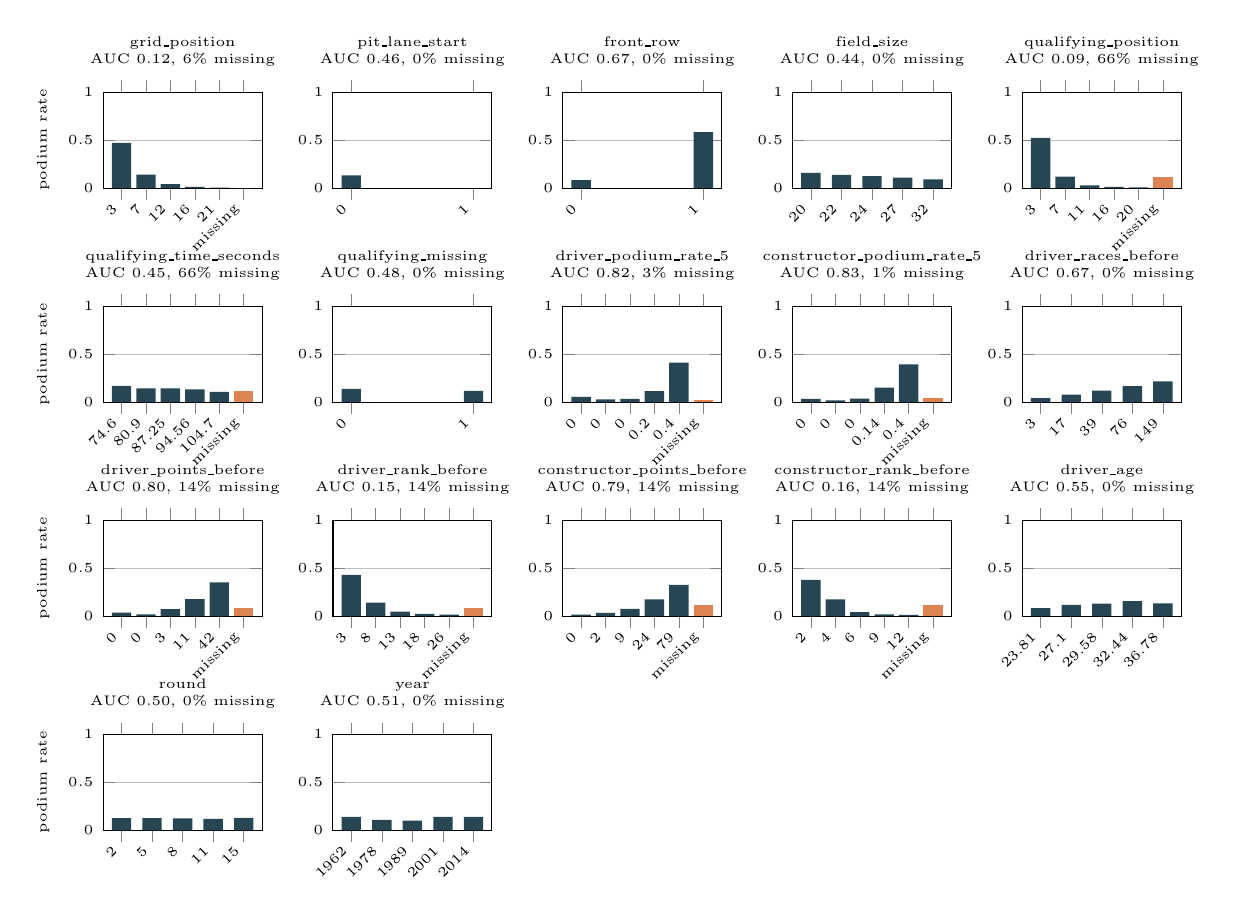
\begin{tikzpicture}
\begin{groupplot}[group style={group size=5 by 4, horizontal sep=0.9cm, vertical sep=1.5cm}, width=3.6cm, height=2.8cm, ymajorgrids, tick label style={font=\tiny}, label style={font=\tiny}]
\nextgroupplot[ybar, bar width=7pt, title={grid\_position\\AUC 0.12, 6\% missing}, title style={align=center, font=\tiny}, xtick={0,1,2,3,4,5}, xticklabels={3,7,12,16,21,missing}, xticklabel style={rotate=45, anchor=east, font=\tiny}, ymin=0, ymax=1, ytick={0,0.5,1}, enlarge x limits=0.15, ylabel={podium rate}]
\addplot[ybar, bar shift=0pt, fill=splitA, draw=none] coordinates {(0,0.470921) (1,0.139434) (2,0.0420479) (3,0.0119826) (4,0.00522876)};
\addplot[ybar, bar shift=0pt, fill=modelB, draw=none] coordinates {(5,0)};
\nextgroupplot[ybar, bar width=7pt, title={pit\_lane\_start\\AUC 0.46, 0\% missing}, title style={align=center, font=\tiny}, xtick={0,1}, xticklabels={0,1}, xticklabel style={rotate=45, anchor=east, font=\tiny}, ymin=0, ymax=1, ytick={0,0.5,1}, enlarge x limits=0.15]
\addplot[ybar, bar shift=0pt, fill=splitA, draw=none] coordinates {(0,0.133938) (1,0)};
\nextgroupplot[ybar, bar width=7pt, title={front\_row\\AUC 0.67, 0\% missing}, title style={align=center, font=\tiny}, xtick={0,1}, xticklabels={0,1}, xticklabel style={rotate=45, anchor=east, font=\tiny}, ymin=0, ymax=1, ytick={0,0.5,1}, enlarge x limits=0.15]
\addplot[ybar, bar shift=0pt, fill=splitA, draw=none] coordinates {(0,0.0838704) (1,0.584729)};
\nextgroupplot[ybar, bar width=7pt, title={field\_size\\AUC 0.44, 0\% missing}, title style={align=center, font=\tiny}, xtick={0,1,2,3,4}, xticklabels={20,22,24,27,32}, xticklabel style={rotate=45, anchor=east, font=\tiny}, ymin=0, ymax=1, ytick={0,0.5,1}, enlarge x limits=0.15]
\addplot[ybar, bar shift=0pt, fill=splitA, draw=none] coordinates {(0,0.158785) (1,0.139013) (2,0.125994) (3,0.110681) (4,0.0921321)};
\nextgroupplot[ybar, bar width=7pt, title={qualifying\_position\\AUC 0.09, 66\% missing}, title style={align=center, font=\tiny}, xtick={0,1,2,3,4,5}, xticklabels={3,7,11,16,20,missing}, xticklabel style={rotate=45, anchor=east, font=\tiny}, ymin=0, ymax=1, ytick={0,0.5,1}, enlarge x limits=0.15]
\addplot[ybar, bar shift=0pt, fill=splitA, draw=none] coordinates {(0,0.524522) (1,0.120886) (2,0.0293238) (3,0.0131658) (4,0.00658288)};
\addplot[ybar, bar shift=0pt, fill=modelB, draw=none] coordinates {(5,0.118284)};
\nextgroupplot[ybar, bar width=7pt, title={qualifying\_time\_seconds\\AUC 0.45, 66\% missing}, title style={align=center, font=\tiny}, xtick={0,1,2,3,4,5}, xticklabels={74.6,80.9,87.25,94.56,104.7,missing}, xticklabel style={rotate=45, anchor=east, font=\tiny}, ymin=0, ymax=1, ytick={0,0.5,1}, enlarge x limits=0.15, ylabel={podium rate}]
\addplot[ybar, bar shift=0pt, fill=splitA, draw=none] coordinates {(0,0.170821) (1,0.144769) (2,0.144161) (3,0.133212) (4,0.107664)};
\addplot[ybar, bar shift=0pt, fill=modelB, draw=none] coordinates {(5,0.117856)};
\nextgroupplot[ybar, bar width=7pt, title={qualifying\_missing\\AUC 0.48, 0\% missing}, title style={align=center, font=\tiny}, xtick={0,1}, xticklabels={0,1}, xticklabel style={rotate=45, anchor=east, font=\tiny}, ymin=0, ymax=1, ytick={0,0.5,1}, enlarge x limits=0.15]
\addplot[ybar, bar shift=0pt, fill=splitA, draw=none] coordinates {(0,0.138942) (1,0.118284)};
\nextgroupplot[ybar, bar width=7pt, title={driver\_podium\_rate\_5\\AUC 0.82, 3\% missing}, title style={align=center, font=\tiny}, xtick={0,1,2,3,4,5}, xticklabels={0,0,0,0.2,0.4,missing}, xticklabel style={rotate=45, anchor=east, font=\tiny}, ymin=0, ymax=1, ytick={0,0.5,1}, enlarge x limits=0.15]
\addplot[ybar, bar shift=0pt, fill=splitA, draw=none] coordinates {(0,0.0542537) (1,0.0280828) (2,0.0344172) (3,0.114443) (4,0.413342)};
\addplot[ybar, bar shift=0pt, fill=modelB, draw=none] coordinates {(5,0.0247934)};
\nextgroupplot[ybar, bar width=7pt, title={constructor\_podium\_rate\_5\\AUC 0.83, 1\% missing}, title style={align=center, font=\tiny}, xtick={0,1,2,3,4,5}, xticklabels={0,0,0,0.14,0.4,missing}, xticklabel style={rotate=45, anchor=east, font=\tiny}, ymin=0, ymax=1, ytick={0,0.5,1}, enlarge x limits=0.15]
\addplot[ybar, bar shift=0pt, fill=splitA, draw=none] coordinates {(0,0.034105) (1,0.0175692) (2,0.0359727) (3,0.150682) (4,0.393758)};
\addplot[ybar, bar shift=0pt, fill=modelB, draw=none] coordinates {(5,0.0470588)};
\nextgroupplot[ybar, bar width=7pt, title={driver\_races\_before\\AUC 0.67, 0\% missing}, title style={align=center, font=\tiny}, xtick={0,1,2,3,4}, xticklabels={3,17,39,76,149}, xticklabel style={rotate=45, anchor=east, font=\tiny}, ymin=0, ymax=1, ytick={0,0.5,1}, enlarge x limits=0.15]
\addplot[ybar, bar shift=0pt, fill=splitA, draw=none] coordinates {(0,0.0430086) (1,0.0786792) (2,0.119878) (3,0.167754) (4,0.217285)};
\nextgroupplot[ybar, bar width=7pt, title={driver\_points\_before\\AUC 0.80, 14\% missing}, title style={align=center, font=\tiny}, xtick={0,1,2,3,4,5}, xticklabels={0,0,3,11,42,missing}, xticklabel style={rotate=45, anchor=east, font=\tiny}, ymin=0, ymax=1, ytick={0,0.5,1}, enlarge x limits=0.15, ylabel={podium rate}]
\addplot[ybar, bar shift=0pt, fill=splitA, draw=none] coordinates {(0,0.0371783) (1,0.0181125) (2,0.0745949) (3,0.17898) (4,0.352002)};
\addplot[ybar, bar shift=0pt, fill=modelB, draw=none] coordinates {(5,0.0848126)};
\nextgroupplot[ybar, bar width=7pt, title={driver\_rank\_before\\AUC 0.15, 14\% missing}, title style={align=center, font=\tiny}, xtick={0,1,2,3,4,5}, xticklabels={3,8,13,18,26,missing}, xticklabel style={rotate=45, anchor=east, font=\tiny}, ymin=0, ymax=1, ytick={0,0.5,1}, enlarge x limits=0.15]
\addplot[ybar, bar shift=0pt, fill=splitA, draw=none] coordinates {(0,0.429695) (1,0.142278) (2,0.0479028) (3,0.0233556) (4,0.0176358)};
\addplot[ybar, bar shift=0pt, fill=modelB, draw=none] coordinates {(5,0.0848126)};
\nextgroupplot[ybar, bar width=7pt, title={constructor\_points\_before\\AUC 0.79, 14\% missing}, title style={align=center, font=\tiny}, xtick={0,1,2,3,4,5}, xticklabels={0,2,9,24,79,missing}, xticklabel style={rotate=45, anchor=east, font=\tiny}, ymin=0, ymax=1, ytick={0,0.5,1}, enlarge x limits=0.15]
\addplot[ybar, bar shift=0pt, fill=splitA, draw=none] coordinates {(0,0.0153992) (1,0.0350628) (2,0.0777251) (3,0.174366) (4,0.327411)};
\addplot[ybar, bar shift=0pt, fill=modelB, draw=none] coordinates {(5,0.121168)};
\nextgroupplot[ybar, bar width=7pt, title={constructor\_rank\_before\\AUC 0.16, 14\% missing}, title style={align=center, font=\tiny}, xtick={0,1,2,3,4,5}, xticklabels={2,4,6,9,12,missing}, xticklabel style={rotate=45, anchor=east, font=\tiny}, ymin=0, ymax=1, ytick={0,0.5,1}, enlarge x limits=0.15]
\addplot[ybar, bar shift=0pt, fill=splitA, draw=none] coordinates {(0,0.379294) (1,0.175551) (2,0.0417062) (3,0.0187159) (4,0.0146885)};
\addplot[ybar, bar shift=0pt, fill=modelB, draw=none] coordinates {(5,0.121168)};
\nextgroupplot[ybar, bar width=7pt, title={driver\_age\\AUC 0.55, 0\% missing}, title style={align=center, font=\tiny}, xtick={0,1,2,3,4}, xticklabels={23.81,27.1,29.58,32.44,36.78}, xticklabel style={rotate=45, anchor=east, font=\tiny}, ymin=0, ymax=1, ytick={0,0.5,1}, enlarge x limits=0.15]
\addplot[ybar, bar shift=0pt, fill=splitA, draw=none] coordinates {(0,0.0847941) (1,0.118834) (2,0.13211) (3,0.157766) (4,0.133102)};
\nextgroupplot[ybar, bar width=7pt, title={round\\AUC 0.50, 0\% missing}, title style={align=center, font=\tiny}, xtick={0,1,2,3,4}, xticklabels={2,5,8,11,15}, xticklabel style={rotate=45, anchor=east, font=\tiny}, ymin=0, ymax=1, ytick={0,0.5,1}, enlarge x limits=0.15, ylabel={podium rate}]
\addplot[ybar, bar shift=0pt, fill=splitA, draw=none] coordinates {(0,0.127191) (1,0.126172) (2,0.125178) (3,0.119649) (4,0.128414)};
\nextgroupplot[ybar, bar width=7pt, title={year\\AUC 0.51, 0\% missing}, title style={align=center, font=\tiny}, xtick={0,1,2,3,4}, xticklabels={1962,1978,1989,2001,2014}, xticklabel style={rotate=45, anchor=east, font=\tiny}, ymin=0, ymax=1, ytick={0,0.5,1}, enlarge x limits=0.15]
\addplot[ybar, bar shift=0pt, fill=splitA, draw=none] coordinates {(0,0.13881) (1,0.108439) (2,0.101121) (3,0.138606) (4,0.139625)};
\end{groupplot}
\end{tikzpicture}}
\caption{Podium rate by feature value on the training seasons. Each bar is one of five equal-count bins (labelled by its median value; tied values are split across bins, so a label can repeat), flags show 0 and 1, and the orange bar is the podium rate of the rows where the feature is missing.}
\end{figure}


\begin{table}[H]
\centering
\caption{One-feature evidence on the training seasons. Missing cells are left out of the bins and the AUC. Valid. is the same AUC on 2020-2021.}
{\footnotesize\rowcolors{2}{white}{zebra}
\begin{tabular}{>{\raggedright\arraybackslash}p{\dimexpr(\linewidth-14\tabcolsep)*291/1000\relax}>{\raggedright\arraybackslash}p{\dimexpr(\linewidth-14\tabcolsep)*127/1000\relax}>{\raggedleft\arraybackslash}p{\dimexpr(\linewidth-14\tabcolsep)*97/1000\relax}>{\raggedleft\arraybackslash}p{\dimexpr(\linewidth-14\tabcolsep)*119/1000\relax}>{\raggedleft\arraybackslash}p{\dimexpr(\linewidth-14\tabcolsep)*127/1000\relax}>{\raggedleft\arraybackslash}p{\dimexpr(\linewidth-14\tabcolsep)*119/1000\relax}>{\raggedleft\arraybackslash}p{\dimexpr(\linewidth-14\tabcolsep)*119/1000\relax}}
\toprule
\rowcolor{navy}
\textcolor{white}{\textbf{Feature}} & \textcolor{white}{\textbf{Group}} & \textcolor{white}{\textbf{Missing}} & \textcolor{white}{\textbf{Lowest bin}} & \textcolor{white}{\textbf{Highest bin}} & \textcolor{white}{\textbf{AUC train}} & \textcolor{white}{\textbf{AUC valid.}} \\
\midrule
grid\_position & grid & 6\% & 47.1\% & 0.5\% & 0.12 & 0.09 \\
pit\_lane\_start & grid & 0\% & 13.4\% & 0.0\% & 0.46 & 0.49 \\
front\_row & grid & 0\% & 8.4\% & 58.5\% & 0.67 & 0.73 \\
field\_size & grid & 0\% & 15.9\% & 9.2\% & 0.44 & 0.50 \\
qualifying\_position & qualifying & 66\% & 52.5\% & 0.7\% & 0.09 & 0.08 \\
qualifying\_time\_seconds & qualifying & 66\% & 17.1\% & 10.8\% & 0.45 & 0.46 \\
qualifying\_missing & qualifying & 0\% & 13.9\% & 11.8\% & 0.48 & 0.50 \\
driver\_podium\_rate\_5 & form & 3\% & 5.4\% & 41.3\% & 0.82 & 0.84 \\
constructor\_podium\_rate\_5 & form & 1\% & 3.4\% & 39.4\% & 0.83 & 0.85 \\
driver\_races\_before & form & 0\% & 4.3\% & 21.7\% & 0.67 & 0.70 \\
driver\_points\_before & standings & 14\% & 3.7\% & 35.2\% & 0.80 & 0.83 \\
driver\_rank\_before & standings & 14\% & 43.0\% & 1.8\% & 0.15 & 0.11 \\
constructor\_points\_before & standings & 14\% & 1.5\% & 32.7\% & 0.79 & 0.82 \\
constructor\_rank\_before & standings & 14\% & 37.9\% & 1.5\% & 0.16 & 0.12 \\
driver\_age & context & 0\% & 8.5\% & 13.3\% & 0.55 & 0.60 \\
round & context & 0\% & 12.7\% & 12.8\% & 0.50 & 0.50 \\
year & context & 0\% & 13.9\% & 14.0\% & 0.51 & 0.50 \\
\bottomrule
\end{tabular}}
\end{table}


\textbf{Strong single signals.} Position features carry the most. Qualifying position has an AUC of 0.09 (lower is better, measured on the third of rows that have it) and grid position 0.12; the podium rate falls from about 45-50\% in the best bin to under 1\% in the worst. The standings ranks (0.15 and 0.16), the form rates (0.82 and 0.83), and the points (0.80 and 0.79) come next. The front-row flag (0.67) and prior starts (0.67) are clear but smaller. All of these keep their direction on validation, with similar or slightly stronger AUCs.


\textbf{Weak single signals, kept for another reason.} Field size (0.44), driver age (0.55), qualifying time (0.45), the pit-lane flag (0.46), and the qualifying-missing flag (0.48) are close to 0.5 on their own. A raw qualifying time is not comparable across circuits and eras, so it says little without the rest of the row. The two flags are indicators. Removing the qualifying-missing flag costs the network 0.041 PR-AUC (Section 6.4), and rows with no grid position, drivers who never started, never podium, while rows with no qualifying record podium at about the average rate (11.8\% against 12.7\%). Round (0.50) and year (0.51) have essentially no single-feature signal, and field size, round, and year are flat or constant on validation, where every race has 20 starters. We keep them as context and era controls, and the ablation shows the whole context group adds the least of the five (0.004 PR-AUC). We have not shown that round or year help on their own, so they are the first candidates to remove.


\begin{takeaway}
\textbf{What this does and does not show.} A one-feature AUC ignores the other 16 features. A feature that looks weak here can still help in combination, and a strong one can add little once the grid is present: the ablation shows qualifying adds only 0.005 on top of the grid. The AUCs describe association in past races, not causes.
\end{takeaway}



\section{Feature engineering and preprocessing: strategy, effect on the values, and order}


Missing qualifying and missing early-season standings have to be filled inside the model pipeline, using training rows only. We compare three settings of logistic regression on the validation seasons: median imputation with scaling, median imputation without scaling, and filling missing values with zero before scaling. The test seasons are not used for this choice.


\begin{table}[H]
\centering
\caption{Preprocessing comparison for logistic regression on 2020-2021 only.}
{\small\rowcolors{2}{white}{zebra}
\begin{tabular}{>{\raggedright\arraybackslash}p{\dimexpr(\linewidth-6\tabcolsep)*366/1000\relax}>{\raggedleft\arraybackslash}p{\dimexpr(\linewidth-6\tabcolsep)*321/1000\relax}>{\raggedleft\arraybackslash}p{\dimexpr(\linewidth-6\tabcolsep)*313/1000\relax}}
\toprule
\rowcolor{navy}
\textcolor{white}{\textbf{Preprocessing}} & \textcolor{white}{\textbf{Validation ROC-AUC}} & \textcolor{white}{\textbf{Validation PR-AUC}} \\
\midrule
median + scaling & 0.926 & 0.728 \\
median, no scaling & 0.924 & 0.724 \\
zero + scaling & 0.927 & 0.725 \\
\bottomrule
\end{tabular}}
\end{table}


We can see that the three PR-AUC values sit between 0.724 and 0.728. The gap is 0.004. Median imputation with scaling is the best of the three on the metric we care about. Zero-filling with scaling is slightly higher on ROC-AUC (0.927 against 0.926). If we had followed ROC-AUC, we would have picked a different setting. The difference is small enough that we do not treat preprocessing as the main lever. We keep median imputation with scaling for the linear model and the network. The forest does not use scaling, because a tree split does not depend on the units of a feature.



\subsection{What feature engineering does to the values}


In Table 14 we compare each raw source column with the feature we built from it. Raw grid has a minimum of 0 and 6.1\% zeros, which would rank a pit-lane start ahead of pole. In the grid-position feature those zeros become missing, so the minimum is 1, and the pit-lane flag carries the information instead. Qualifying strings become seconds; after the join to every driver-race row, 61.2\% of rows have no qualifying time. Shifted form and previous-race standings are missing on a first race or first round, because nothing earlier exists. These gaps are what the imputer fills next.


\begin{table}[H]
\centering
\caption{Raw source columns against the engineered features built from them (all 1950-2024 rows).}
{\small\rowcolors{2}{white}{zebra}
\begin{tabular}{>{\raggedright\arraybackslash}p{\dimexpr(\linewidth-12\tabcolsep)*372/1000\relax}>{\raggedleft\arraybackslash}p{\dimexpr(\linewidth-12\tabcolsep)*117/1000\relax}>{\raggedleft\arraybackslash}p{\dimexpr(\linewidth-12\tabcolsep)*102/1000\relax}>{\raggedleft\arraybackslash}p{\dimexpr(\linewidth-12\tabcolsep)*124/1000\relax}>{\raggedleft\arraybackslash}p{\dimexpr(\linewidth-12\tabcolsep)*139/1000\relax}>{\raggedleft\arraybackslash}p{\dimexpr(\linewidth-12\tabcolsep)*146/1000\relax}}
\toprule
\rowcolor{navy}
\textcolor{white}{\textbf{Column}} & \textcolor{white}{\textbf{Missing}} & \textcolor{white}{\textbf{Zeros}} & \textcolor{white}{\textbf{Min}} & \textcolor{white}{\textbf{Median}} & \textcolor{white}{\textbf{Max}} \\
\midrule
grid (raw) & 0.0\% & 6.1\% & 0.00 & 11.00 & 34.00 \\
grid\_position (0 $\rightarrow$ missing) & 6.1\% & 0.0\% & 1.00 & 12.00 & 34.00 \\
pit\_lane\_start (grid == 0) & 0.0\% & 93.9\% & 0.00 & 0.00 & 1.00 \\
q1/q2/q3 text present & 0.0\% & 1.5\% & 0.00 & 1.00 & 1.00 \\
best qualifying seconds (parsed) & 1.5\% & 0.0\% & 53.38 & 86.69 & 1002.64 \\
qualifying\_time\_seconds (joined) & 61.2\% & 0.0\% & 53.38 & 86.69 & 1002.64 \\
driver\_podium\_rate\_5 (shifted) & 3.2\% & 66.3\% & 0.00 & 0.00 & 1.00 \\
driver\_points\_before (previous race) & 13.7\% & 29.5\% & 0.00 & 4.00 & 549.00 \\
\bottomrule
\end{tabular}}
\end{table}



\subsection{What imputation and scaling do to the values}


In Table 15 we measure both steps on the training rows. Median imputation writes the training median into every gap. It does not change the range, because the median is inside it, but it piles rows onto one value and shrinks the spread. qualifying\_time\_seconds is missing in 66.5\% of training rows, and its standard deviation falls by 41.9\%. The qualifying-missing flag keeps the fact that a value was filled. Scaling then puts every training feature at mean 0 and standard deviation 1. Raw ranges run from 0-1 for the flags to 722 constructor points; after scaling they share one scale, so neither the logistic penalty nor the network's gradient steps are dominated by large units. Scaling is linear, so the shape and order of values do not change.


\begin{table}[H]
\centering
\caption{Effect of median imputation and scaling, fitted on 1950-2019. Val. and test means are after the same training-fitted transform; training means are 0 by construction.}
{\footnotesize\rowcolors{2}{white}{zebra}
\begin{tabular}{>{\raggedright\arraybackslash}p{\dimexpr(\linewidth-16\tabcolsep)*232/1000\relax}>{\raggedleft\arraybackslash}p{\dimexpr(\linewidth-16\tabcolsep)*87/1000\relax}>{\raggedleft\arraybackslash}p{\dimexpr(\linewidth-16\tabcolsep)*101/1000\relax}>{\raggedleft\arraybackslash}p{\dimexpr(\linewidth-16\tabcolsep)*152/1000\relax}>{\raggedleft\arraybackslash}p{\dimexpr(\linewidth-16\tabcolsep)*101/1000\relax}>{\raggedleft\arraybackslash}p{\dimexpr(\linewidth-16\tabcolsep)*145/1000\relax}>{\raggedleft\arraybackslash}p{\dimexpr(\linewidth-16\tabcolsep)*87/1000\relax}>{\raggedleft\arraybackslash}p{\dimexpr(\linewidth-16\tabcolsep)*94/1000\relax}}
\toprule
\rowcolor{navy}
\textcolor{white}{\textbf{Feature}} & \textcolor{white}{\textbf{Missing}} & \textcolor{white}{\textbf{Fill value}} & \textcolor{white}{\textbf{Raw range}} & \textcolor{white}{\textbf{Std change}} & \textcolor{white}{\textbf{Scaled range}} & \textcolor{white}{\textbf{Val. mean}} & \textcolor{white}{\textbf{Test mean}} \\
\midrule
grid\_position & 6.4\% & 12.00 & 1.0 to 34.0 & $-$3.3\% & $-$1.65 to 3.29 & $-$0.24 & $-$0.26 \\
qualifying\_position & 65.9\% & 11.00 & 1.0 to 28.0 & $-$41.6\% & $-$2.72 to 4.53 & $-$0.17 & $-$0.17 \\
qualifying\_time\_seconds & 66.5\% & 87.25 & 63.0 to 1002.6 & $-$41.9\% & $-$2.71 to 99.99 & $-$0.46 & $-$0.26 \\
driver\_podium\_rate\_5 & 3.5\% & 0.00 & 0.0 to 1.0 & $-$1.2\% & $-$0.55 to 3.88 & +0.11 & +0.12 \\
driver\_points\_before & 14.5\% & 3.00 & 0.0 to 387.0 & $-$6.7\% & $-$0.42 to 11.18 & +0.99 & +1.35 \\
constructor\_points\_before & 14.0\% & 9.00 & 0.0 to 722.0 & $-$6.5\% & $-$0.45 to 10.76 & +1.03 & +1.39 \\
driver\_age & 0.0\% & 29.58 & 17.5 to 58.8 & 0.0\% & $-$2.43 to 5.51 & $-$0.43 & $-$0.25 \\
year & 0.0\% & 1989.00 & 1950.0 to 2019.0 & 0.0\% & $-$2.11 to 1.63 & +1.72 & +1.85 \\
\bottomrule
\end{tabular}}
\end{table}


Figure 8 shows the spike at the median and the shift of later seasons; in Figure 9 we compare raw and scaled ranges for all 17 features. Because the transform is fitted on training only, validation and test are not centred at zero: year sits at +1.72 standard deviations in validation. That is the period shift the model faces at deployment, not a bug.


\begin{figure}[H]
\centering
{\scriptsize Top row: \textcolor{modelB}{\rule{1.2ex}{1.2ex}} after median imputation, \textcolor{splitA}{\rule{1.2ex}{1.2ex}} observed values, dashed line = fill value. Bottom row: \textcolor{modelC}{\rule{1.2ex}{1.2ex}} training, \textcolor{splitB}{\rule{1.2ex}{1.2ex}} validation.\par}\smallskip
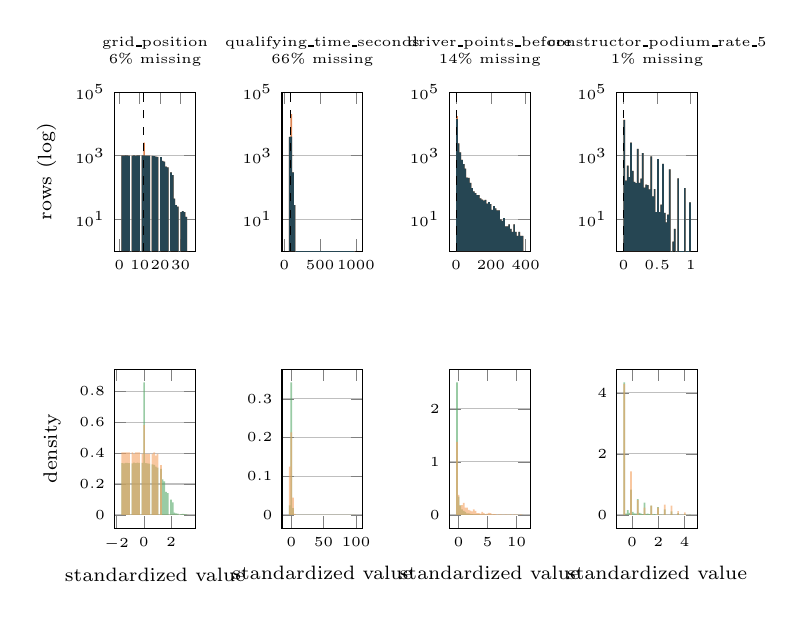
\begin{tikzpicture}
\begin{groupplot}[group style={group size=4 by 2, horizontal sep=1.1cm, vertical sep=1.5cm}, width=0.215\linewidth, height=3.6cm, ymajorgrids, tick label style={font=\tiny}]
\nextgroupplot[title={grid\_position\\6\% missing}, ymode=log, ymin=1, ymax=100000, title style={align=center, font=\tiny}, ylabel={rows (log)}]
\addplot[ybar interval, fill=modelB, draw=none] coordinates {(1,1017) (1.825,1013) (2.65,1020) (3.475,1021) (4.3,1014) (5.125,0.5) (5.95,1013) (6.775,1026) (7.6,1016) (8.425,1025) (9.25,1019) (10.075,0.5) (10.9,1020) (11.725,2598) (12.55,1017) (13.375,1013) (14.2,1005) (15.025,0.5) (15.85,992) (16.675,979) (17.5,946) (18.325,929) (19.15,0.5) (19.975,903) (20.8,696) (21.625,656) (22.45,451) (23.275,429) (24.1,0.5) (24.925,301) (25.75,247) (26.575,45) (27.4,28) (28.225,25) (29.05,0.5) (29.875,17) (30.7,18) (31.525,17) (32.35,12) (33.175,1) (34,1)};
\addplot[ybar interval, fill=splitA, draw=none] coordinates {(1,1017) (1.825,1013) (2.65,1020) (3.475,1021) (4.3,1014) (5.125,0.5) (5.95,1013) (6.775,1026) (7.6,1016) (8.425,1025) (9.25,1019) (10.075,0.5) (10.9,1020) (11.725,1020) (12.55,1017) (13.375,1013) (14.2,1005) (15.025,0.5) (15.85,992) (16.675,979) (17.5,946) (18.325,929) (19.15,0.5) (19.975,903) (20.8,696) (21.625,656) (22.45,451) (23.275,429) (24.1,0.5) (24.925,301) (25.75,247) (26.575,45) (27.4,28) (28.225,25) (29.05,0.5) (29.875,17) (30.7,18) (31.525,17) (32.35,12) (33.175,1) (34,1)};
\addplot[black, dashed] coordinates {(12,1) (12,100000)};
\nextgroupplot[title={qualifying\_time\_seconds\\66\% missing}, ymode=log, ymin=1, ymax=100000, title style={align=center, font=\tiny}]
\addplot[ybar interval, fill=modelB, draw=none] coordinates {(63.003,3915) (86.4939,20284) (109.985,301) (133.476,28) (156.967,0.5) (180.458,0.5) (203.949,0.5) (227.439,0.5) (250.93,0.5) (274.421,0.5) (297.912,0.5) (321.403,0.5) (344.894,0.5) (368.385,0.5) (391.876,0.5) (415.367,0.5) (438.858,0.5) (462.349,0.5) (485.84,0.5) (509.331,0.5) (532.822,0.5) (556.312,0.5) (579.803,0.5) (603.294,0.5) (626.785,0.5) (650.276,0.5) (673.767,0.5) (697.258,0.5) (720.749,0.5) (744.24,0.5) (767.731,0.5) (791.222,0.5) (814.713,0.5) (838.204,0.5) (861.694,0.5) (885.185,0.5) (908.676,0.5) (932.167,0.5) (955.658,0.5) (979.149,1) (1002.64,1)};
\addplot[ybar interval, fill=splitA, draw=none] coordinates {(63.003,3915) (86.4939,3976) (109.985,301) (133.476,28) (156.967,0.5) (180.458,0.5) (203.949,0.5) (227.439,0.5) (250.93,0.5) (274.421,0.5) (297.912,0.5) (321.403,0.5) (344.894,0.5) (368.385,0.5) (391.876,0.5) (415.367,0.5) (438.858,0.5) (462.349,0.5) (485.84,0.5) (509.331,0.5) (532.822,0.5) (556.312,0.5) (579.803,0.5) (603.294,0.5) (626.785,0.5) (650.276,0.5) (673.767,0.5) (697.258,0.5) (720.749,0.5) (744.24,0.5) (767.731,0.5) (791.222,0.5) (814.713,0.5) (838.204,0.5) (861.694,0.5) (885.185,0.5) (908.676,0.5) (932.167,0.5) (955.658,0.5) (979.149,1) (1002.64,1)};
\addplot[black, dashed] coordinates {(87.249,1) (87.249,100000)};
\nextgroupplot[title={driver\_points\_before\\14\% missing}, ymode=log, ymin=1, ymax=100000, title style={align=center, font=\tiny}]
\addplot[ybar interval, fill=modelB, draw=none] coordinates {(0,17756) (9.675,2448) (19.35,1283) (29.025,741) (38.7,548) (48.375,397) (58.05,206) (67.725,203) (77.4,140) (87.075,96) (96.75,76) (106.425,67) (116.1,58) (125.775,58) (135.45,46) (145.125,42) (154.8,39) (164.475,41) (174.15,31) (183.825,35) (193.5,30) (203.175,20) (212.85,26) (222.525,22) (232.2,19) (241.875,19) (251.55,10) (261.225,9) (270.9,11) (280.575,6) (290.25,6) (299.925,7) (309.6,5) (319.275,4) (328.95,7) (338.625,4) (348.3,3) (357.975,4) (367.65,3) (377.325,3) (387,3)};
\addplot[ybar interval, fill=splitA, draw=none] coordinates {(0,14207) (9.675,2448) (19.35,1283) (29.025,741) (38.7,548) (48.375,397) (58.05,206) (67.725,203) (77.4,140) (87.075,96) (96.75,76) (106.425,67) (116.1,58) (125.775,58) (135.45,46) (145.125,42) (154.8,39) (164.475,41) (174.15,31) (183.825,35) (193.5,30) (203.175,20) (212.85,26) (222.525,22) (232.2,19) (241.875,19) (251.55,10) (261.225,9) (270.9,11) (280.575,6) (290.25,6) (299.925,7) (309.6,5) (319.275,4) (328.95,7) (338.625,4) (348.3,3) (357.975,4) (367.65,3) (377.325,3) (387,3)};
\addplot[black, dashed] coordinates {(3,1) (3,100000)};
\nextgroupplot[title={constructor\_podium\_rate\_5\\1\% missing}, ymode=log, ymin=1, ymax=100000, title style={align=center, font=\tiny}]
\addplot[ybar interval, fill=modelB, draw=none] coordinates {(0,13594) (0.025,165) (0.05,492) (0.075,211) (0.1,2578) (0.125,337) (0.15,151) (0.175,138) (0.2,1632) (0.225,139) (0.25,192) (0.275,1221) (0.3,99) (0.325,123) (0.35,119) (0.375,87) (0.4,961) (0.425,53) (0.45,89) (0.475,17) (0.5,788) (0.525,17) (0.55,29) (0.575,556) (0.6,16) (0.625,8) (0.65,14) (0.675,372) (0.7,0.5) (0.725,2) (0.75,5) (0.775,0.5) (0.8,194) (0.825,0.5) (0.85,0.5) (0.875,0.5) (0.9,96) (0.925,0.5) (0.95,0.5) (0.975,34) (1,34)};
\addplot[ybar interval, fill=splitA, draw=none] coordinates {(0,13254) (0.025,165) (0.05,492) (0.075,211) (0.1,2578) (0.125,337) (0.15,151) (0.175,138) (0.2,1632) (0.225,139) (0.25,192) (0.275,1221) (0.3,99) (0.325,123) (0.35,119) (0.375,87) (0.4,961) (0.425,53) (0.45,89) (0.475,17) (0.5,788) (0.525,17) (0.55,29) (0.575,556) (0.6,16) (0.625,8) (0.65,14) (0.675,372) (0.7,0.5) (0.725,2) (0.75,5) (0.775,0.5) (0.8,194) (0.825,0.5) (0.85,0.5) (0.875,0.5) (0.9,96) (0.925,0.5) (0.95,0.5) (0.975,34) (1,34)};
\addplot[black, dashed] coordinates {(0,1) (0,100000)};
\nextgroupplot[xlabel={standardized value}, ylabel={density}]
\addplot[ybar interval, fill=modelC, fill opacity=0.6, draw=none] coordinates {(-1.64934,0.335509) (-1.52576,0.334189) (-1.40219,0.336498) (-1.27861,0.336828) (-1.15503,0.334519) (-1.03146,0) (-0.90788,0.334189) (-0.784303,0.338478) (-0.660726,0.335179) (-0.537149,0.338148) (-0.413572,0.336168) (-0.289995,0) (-0.166418,0.336498) (-0.0428411,0.857081) (0.0807358,0.335509) (0.204313,0.334189) (0.32789,0.33155) (0.451467,0) (0.575044,0.327261) (0.698621,0.322972) (0.822198,0.312086) (0.945775,0.306477) (1.06935,0) (1.19293,0.2979) (1.31651,0.229611) (1.44008,0.216415) (1.56366,0.148785) (1.68724,0.141527) (1.81081,0) (1.93439,0.0993) (2.05797,0.0814854) (2.18154,0.0148455) (2.30512,0.00923721) (2.4287,0.00824751) (2.55227,0) (2.67585,0.0056083) (2.79943,0.0059382) (2.92301,0.0056083) (3.04658,0.0039588) (3.17016,0.0003299) (3.29374,0.0003299)};
\addplot[ybar interval, fill=splitB, fill opacity=0.6, draw=none] coordinates {(-1.64934,0.404606) (-1.52576,0.404606) (-1.40219,0.404606) (-1.27861,0.404606) (-1.15503,0.404606) (-1.03146,0) (-0.90788,0.404606) (-0.784303,0.394232) (-0.660726,0.404606) (-0.537149,0.404606) (-0.413572,0.404606) (-0.289995,0) (-0.166418,0.394232) (-0.0428411,0.580973) (0.0807358,0.394232) (0.204313,0.394232) (0.32789,0.394232) (0.451467,0) (0.575044,0.394232) (0.698621,0.404606) (0.822198,0.383857) (0.945775,0.394232) (1.06935,0) (1.19293,0.32161) (1.31651,0) (1.44008,0) (1.56366,0) (1.68724,0) (1.81081,0) (1.93439,0) (2.05797,0) (2.18154,0) (2.30512,0) (2.4287,0) (2.55227,0) (2.67585,0) (2.79943,0) (2.92301,0) (3.04658,0) (3.17016,0) (3.29374,0)};
\nextgroupplot[xlabel={standardized value}]
\addplot[ybar interval, fill=modelC, fill opacity=0.6, draw=none] coordinates {(-3.7582,0.0244263) (-1.16454,0.342219) (1.42913,0.0178089) (4.0228,0.00102169) (6.61646,6.28733e-05) (9.21013,0) (11.8038,0) (14.3975,0) (16.9911,0) (19.5848,0) (22.1785,0) (24.7721,0) (27.3658,0) (29.9594,0) (32.5531,0) (35.1468,0) (37.7404,0) (40.3341,0) (42.9278,0) (45.5214,0) (48.1151,0) (50.7088,0) (53.3024,0) (55.8961,0) (58.4898,0) (61.0834,0) (63.6771,0) (66.2708,0) (68.8644,0) (71.4581,0) (74.0518,0) (76.6454,0) (79.2391,0) (81.8328,0) (84.4264,0) (87.0201,0) (89.6138,0) (92.2074,0) (94.8011,0) (97.3947,1.57183e-05) (99.9884,1.57183e-05)};
\addplot[ybar interval, fill=splitB, fill opacity=0.6, draw=none] coordinates {(-3.7582,0.124564) (-1.16454,0.213044) (1.42913,0.0449814) (4.0228,0.00296581) (6.61646,0) (9.21013,0) (11.8038,0) (14.3975,0) (16.9911,0) (19.5848,0) (22.1785,0) (24.7721,0) (27.3658,0) (29.9594,0) (32.5531,0) (35.1468,0) (37.7404,0) (40.3341,0) (42.9278,0) (45.5214,0) (48.1151,0) (50.7088,0) (53.3024,0) (55.8961,0) (58.4898,0) (61.0834,0) (63.6771,0) (66.2708,0) (68.8644,0) (71.4581,0) (74.0518,0) (76.6454,0) (79.2391,0) (81.8328,0) (84.4264,0) (87.0201,0) (89.6138,0) (92.2074,0) (94.8011,0) (97.3947,0) (99.9884,0)};
\nextgroupplot[xlabel={standardized value}]
\addplot[ybar interval, fill=modelC, fill opacity=0.6, draw=none] coordinates {(-0.419012,2.49679) (-0.129088,0.34423) (0.160835,0.180411) (0.450759,0.104197) (0.740682,0.0770579) (1.03061,0.0558248) (1.32053,0.028967) (1.61045,0.0285452) (1.90038,0.0196863) (2.1903,0.0134992) (2.48022,0.0106869) (2.77015,0.00942131) (3.06007,0.00815576) (3.34999,0.00815576) (3.63992,0.00646837) (3.92984,0.0059059) (4.21976,0.00548405) (4.50969,0.00576528) (4.79961,0.00435912) (5.08954,0.00492158) (5.37946,0.0042185) (5.66938,0.00281233) (5.95931,0.00365603) (6.24923,0.00309357) (6.53915,0.00267172) (6.82908,0.00267172) (7.119,0.00140617) (7.40892,0.00126555) (7.69885,0.00154678) (7.98877,0.0008437) (8.27869,0.0008437) (8.56862,0.000984316) (8.85854,0.000703083) (9.14846,0.000562467) (9.43839,0.000984316) (9.72831,0.000562467) (10.0182,0.00042185) (10.3082,0.000562467) (10.5981,0.00042185) (10.888,0.00042185) (11.1779,0.00042185)};
\addplot[ybar interval, fill=splitB, fill opacity=0.6, draw=none] coordinates {(-0.419012,1.37525) (-0.129088,0.375873) (0.160835,0.176881) (0.450759,0.185725) (0.740682,0.225524) (1.03061,0.137083) (1.32053,0.137083) (1.61045,0.0972847) (1.90038,0.0795966) (2.1903,0.0663305) (2.48022,0.106129) (2.77015,0.0751746) (3.06007,0.0353763) (3.34999,0.0353763) (3.63992,0.0265322) (3.92984,0.0574864) (4.21976,0.0353763) (4.50969,0.00884407) (4.79961,0.0221102) (5.08954,0.0397983) (5.37946,0.0353763) (5.66938,0.00884407) (5.95931,0.0132661) (6.24923,0.0132661) (6.53915,0) (6.82908,0.00884407) (7.119,0.00884407) (7.40892,0.00442203) (7.69885,0.00442203) (7.98877,0.00884407) (8.27869,0.00442203) (8.56862,0.00442203) (8.85854,0.00884407) (9.14846,0) (9.43839,0.00884407) (9.72831,0.00442203) (10.0182,0.00442203) (10.3082,0) (10.5981,0.00884407) (10.888,0) (11.1779,0)};
\nextgroupplot[xlabel={standardized value}]
\addplot[ybar interval, fill=modelC, fill opacity=0.6, draw=none] coordinates {(-0.650067,4.33837) (-0.52205,0.0433105) (-0.394034,0.155408) (-0.266017,0.0684688) (-0.138001,0.827357) (-0.00998421,0.100952) (0.118032,0.0464951) (0.246049,0.0455397) (0.374065,0.519726) (0.502082,0.0627365) (0.630099,0.0426736) (0.758115,0.0219737) (0.886132,0.398393) (1.01415,0.0337567) (1.14216,0.0433105) (1.27018,0.027706) (1.3982,0.306039) (1.52621,0.0210183) (1.65423,0.0242029) (1.78225,0.00541381) (1.91026,0.250946) (2.03828,0.00541381) (2.1663,0.00923532) (2.29431,0.00477689) (2.42233,0.177382) (2.55035,0.00254767) (2.67836,0.00445843) (2.80638,0) (2.9344,0.118467) (3.06241,0.000636919) (3.19043,0.0015923) (3.31845,0) (3.44646,0.0617811) (3.57448,0) (3.7025,0) (3.83051,0) (3.95853,0.0305721) (4.08655,0) (4.21456,0) (4.34258,0.0108276) (4.4706,0.0108276)};
\addplot[ybar interval, fill=splitB, fill opacity=0.6, draw=none] coordinates {(-0.650067,4.2863) (-0.52205,0) (-0.394034,0) (-0.266017,0) (-0.138001,1.42209) (-0.00998421,0) (0.118032,0) (0.246049,0) (0.374065,0.480707) (0.502082,0) (0.630099,0) (0.758115,0) (0.886132,0.240354) (1.01415,0) (1.14216,0) (1.27018,0) (1.3982,0.300442) (1.52621,0) (1.65423,0) (1.78225,0) (1.91026,0.240354) (2.03828,0) (2.1663,0) (2.29431,0) (2.42233,0.340501) (2.55035,0) (2.67836,0) (2.80638,0) (2.9344,0.300442) (3.06241,0) (3.19043,0) (3.31845,0) (3.44646,0.120177) (3.57448,0) (3.7025,0) (3.83051,0) (3.95853,0.0801178) (4.08655,0) (4.21456,0) (4.34258,0) (4.4706,0)};
\end{groupplot}
\end{tikzpicture}
\caption{Top: training values before and after median imputation (dashed line is the fill value, log scale). Bottom: training and validation after the training-fitted scaler.}
\end{figure}


\begin{figure}[H]
\centering
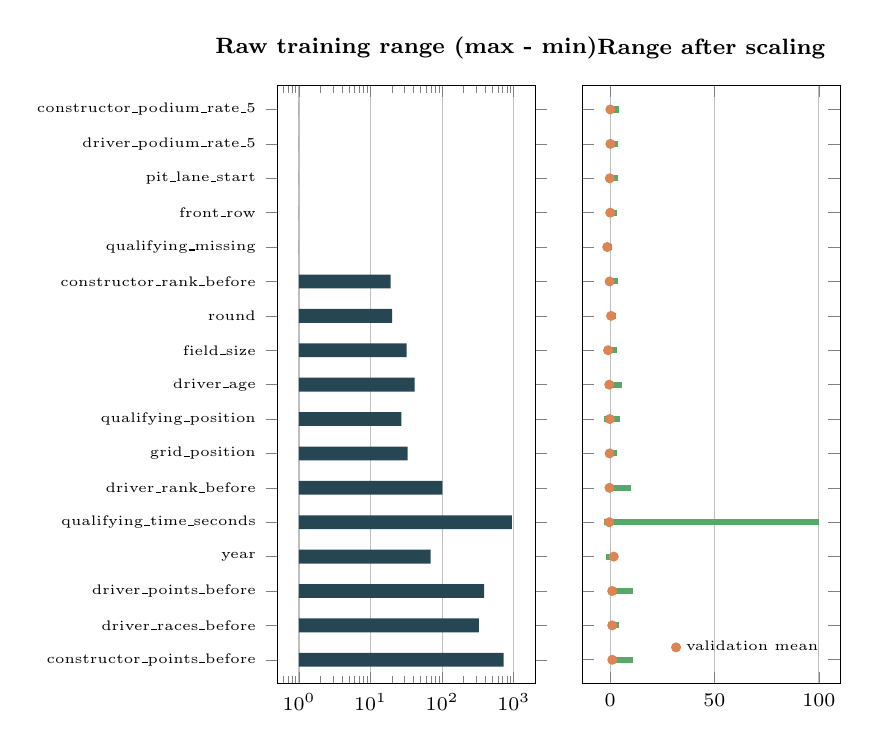
\begin{tikzpicture}
\begin{axis}[name=left, xbar, bar width=5pt, width=0.270\linewidth, xmode=log, xmin=0.5, title={Raw training range (max - min)}, ytick={0,1,2,3,4,5,6,7,8,9,10,11,12,13,14,15,16}, yticklabels={constructor\_podium\_rate\_5,driver\_podium\_rate\_5,pit\_lane\_start,front\_row,qualifying\_missing,constructor\_rank\_before,round,field\_size,driver\_age,qualifying\_position,grid\_position,driver\_rank\_before,qualifying\_time\_seconds,year,driver\_points\_before,driver\_races\_before,constructor\_points\_before}, y dir=reverse, ymin=-0.7, ymax=16.7, height=7.6cm, scale only axis, yticklabel style={font=\tiny}, xmajorgrids]
\addplot[xbar, fill=splitA, draw=none] coordinates {(1,0) (1,1) (1,2) (1,3) (1,4) (19,5) (20,6) (32,7) (41.3342,8) (27,9) (33,10) (101,11) (939.637,12) (69,13) (387,14) (325,15) (722,16)};
\end{axis}
\begin{axis}[at={(left.east)}, anchor=west, xshift=0.6cm, width=0.270\linewidth, title={Range after scaling}, ytick={0,1,2,3,4,5,6,7,8,9,10,11,12,13,14,15,16}, yticklabels={constructor\_podium\_rate\_5,driver\_podium\_rate\_5,pit\_lane\_start,front\_row,qualifying\_missing,constructor\_rank\_before,round,field\_size,driver\_age,qualifying\_position,grid\_position,driver\_rank\_before,qualifying\_time\_seconds,year,driver\_points\_before,driver\_races\_before,constructor\_points\_before}, y dir=reverse, ymin=-0.7, ymax=16.7, height=7.6cm, scale only axis, yticklabel style={font=\tiny}, xmajorgrids, yticklabels=\empty, legend pos=south east, legend style={font=\tiny}]
\addplot[modelC, line width=2.2pt, forget plot] coordinates {(-0.650067,0) (4.4706,0)};
\addplot[modelC, line width=2.2pt, forget plot] coordinates {(-0.546627,1) (3.87774,1)};
\addplot[modelC, line width=2.2pt, forget plot] coordinates {(-0.262212,2) (3.81371,2)};
\addplot[modelC, line width=2.2pt, forget plot] coordinates {(-0.300377,3) (3.32915,3)};
\addplot[modelC, line width=2.2pt, forget plot] coordinates {(-1.39122,4) (0.718793,4)};
\addplot[modelC, line width=2.2pt, forget plot] coordinates {(-1.45695,5) (3.62205,5)};
\addplot[modelC, line width=2.2pt, forget plot] coordinates {(-1.49753,6) (2.61496,6)};
\addplot[modelC, line width=2.2pt, forget plot] coordinates {(-2.95993,7) (3.33136,7)};
\addplot[modelC, line width=2.2pt, forget plot] coordinates {(-2.43154,8) (5.50791,8)};
\addplot[modelC, line width=2.2pt, forget plot] coordinates {(-2.72152,9) (4.53362,9)};
\addplot[modelC, line width=2.2pt, forget plot] coordinates {(-1.64934,10) (3.29374,10)};
\addplot[modelC, line width=2.2pt, forget plot] coordinates {(-1.41544,11) (9.80577,11)};
\addplot[modelC, line width=2.2pt, forget plot] coordinates {(-2.70616,12) (99.9884,12)};
\addplot[modelC, line width=2.2pt, forget plot] coordinates {(-2.10594,13) (1.63441,13)};
\addplot[modelC, line width=2.2pt, forget plot] coordinates {(-0.419012,14) (11.1779,14)};
\addplot[modelC, line width=2.2pt, forget plot] coordinates {(-0.977025,15) (4.33086,15)};
\addplot[modelC, line width=2.2pt, forget plot] coordinates {(-0.447292,16) (10.764,16)};
\addplot[only marks, mark=*, mark size=1.6pt, modelB] coordinates {(0.0930855,0) (0.113626,1) (-0.173378,2) (0.062576,3) (-1.38852,4) (-0.247172,5) (0.437447,6) (-0.993898,7) (-0.430939,8) (-0.171886,9) (-0.243042,10) (-0.32822,11) (-0.463989,12) (1.7192,13) (0.988096,14) (1.00084,15) (1.02689,16)};
\legend{validation mean}
\end{axis}
\end{tikzpicture}
\caption{Left: raw training range per feature. Right: range after scaling, with the validation mean.}
\end{figure}



\subsection{Preprocessing-order experiments}


The table above changes which strategy we use. We also ran three experiments that change the \textit{order} of the steps (Table 16), each scored on validation with logistic regression and the network. A swaps median imputation and scaling. B swaps zero-filling and scaling. C fits the preprocessing on all seasons before splitting, against the normal fit on training only.


\begin{table}[H]
\centering
\caption{Preprocessing-order experiments on 2020-2021. Change is against the first order of the same experiment and model; for C it is against the train-only fit.}
{\footnotesize\rowcolors{2}{white}{zebra}
\begin{tabular}{>{\raggedright\arraybackslash}p{\dimexpr(\linewidth-14\tabcolsep)*119/1000\relax}>{\raggedright\arraybackslash}p{\dimexpr(\linewidth-14\tabcolsep)*214/1000\relax}>{\raggedright\arraybackslash}p{\dimexpr(\linewidth-14\tabcolsep)*119/1000\relax}>{\raggedright\arraybackslash}p{\dimexpr(\linewidth-14\tabcolsep)*103/1000\relax}>{\raggedleft\arraybackslash}p{\dimexpr(\linewidth-14\tabcolsep)*190/1000\relax}>{\raggedleft\arraybackslash}p{\dimexpr(\linewidth-14\tabcolsep)*135/1000\relax}>{\raggedleft\arraybackslash}p{\dimexpr(\linewidth-14\tabcolsep)*119/1000\relax}}
\toprule
\rowcolor{navy}
\textcolor{white}{\textbf{Experiment}} & \textcolor{white}{\textbf{Order}} & \textcolor{white}{\textbf{Fitted on}} & \textcolor{white}{\textbf{Model}} & \textcolor{white}{\textbf{Missing grid becomes}} & \textcolor{white}{\textbf{Val. PR-AUC}} & \textcolor{white}{\textbf{Change}} \\
\midrule
A & impute $\rightarrow$ scale & train & LogReg & 12.00 & 0.728 & +0.0000 \\
A & impute $\rightarrow$ scale & train & MLP & 12.00 & 0.738 & +0.0000 \\
A & scale $\rightarrow$ impute & train & LogReg & 12.00 & 0.728 & +0.0000 \\
A & scale $\rightarrow$ impute & train & MLP & 12.00 & 0.727 & $-$0.0117 \\
B & zero-fill $\rightarrow$ scale & train & LogReg & 0.00 & 0.725 & +0.0000 \\
B & zero-fill $\rightarrow$ scale & train & MLP & 0.00 & 0.701 & +0.0000 \\
B & scale $\rightarrow$ zero-fill & train & LogReg & 12.01 & 0.727 & +0.0020 \\
B & scale $\rightarrow$ zero-fill & train & MLP & 12.01 & 0.711 & +0.0103 \\
C & impute $\rightarrow$ scale & all years & LogReg & 12.00 & 0.727 & $-$0.0002 \\
C & impute $\rightarrow$ scale & all years & MLP & 12.00 & 0.700 & $-$0.0383 \\
\bottomrule
\end{tabular}}
\end{table}


\textbf{A.} Median imputation commutes with a linear rescale, so a missing grid becomes 12.0 either way. Only the scaler's statistics differ, because scaling first measures spread on observed values. Validation PR-AUC moves by +0.0000 for logistic regression and $-$0.0117 for the network. \textbf{B.} Here order changes the value. Zero-filling first writes a literal 0, a grid slot ahead of pole and a 0-second lap. Zero-filling after scaling writes the training mean (12.0 for grid). Validation PR-AUC changes by +0.0020 (logistic) and +0.0103 (network). \textbf{C.} Fitting before the split lets 2020-2024 set the medians and scaling used in training. The score moves by $-$0.0002 and $-$0.0383; small or not, it uses future data, so we never do it.


\begin{takeaway}
\textbf{Takeaway.} We keep split, then median imputation, then scaling, all fitted on training rows inside the model pipeline. Logistic regression is almost indifferent to strategy and order (every change is within 0.004 PR-AUC). The network is more sensitive, up to about 0.04 PR-AUC, so for it the order is part of the model, not a detail. The next sections test which information the models need.
\end{takeaway}



\subsection{Missing values: impute, drop columns, or drop rows?}


About two thirds of training rows have no qualifying record, so we did not choose the handling by preference. Each approach is scored on the same validation seasons (Table 17). The network is run once with one seed, and its seed-to-seed spread is about 0.016 (Section 7.1), so small network differences are noise.


\begin{table}[H]
\centering
\caption{Missing-value experiments on 2020-2021. Change is against median imputation, which is used.}
{\small\rowcolors{2}{white}{zebra}
\begin{tabular}{>{\raggedright\arraybackslash}p{\dimexpr(\linewidth-12\tabcolsep)*453/1000\relax}>{\raggedleft\arraybackslash}p{\dimexpr(\linewidth-12\tabcolsep)*109/1000\relax}>{\raggedleft\arraybackslash}p{\dimexpr(\linewidth-12\tabcolsep)*125/1000\relax}>{\raggedleft\arraybackslash}p{\dimexpr(\linewidth-12\tabcolsep)*94/1000\relax}>{\raggedleft\arraybackslash}p{\dimexpr(\linewidth-12\tabcolsep)*125/1000\relax}>{\raggedleft\arraybackslash}p{\dimexpr(\linewidth-12\tabcolsep)*94/1000\relax}}
\toprule
\rowcolor{navy}
\textcolor{white}{\textbf{Approach}} & \textcolor{white}{\textbf{Training rows}} & \textcolor{white}{\textbf{LogReg PR-AUC}} & \textcolor{white}{\textbf{Change}} & \textcolor{white}{\textbf{MLP PR-AUC}} & \textcolor{white}{\textbf{Change}} \\
\midrule
median imputation (used) & 24,529 & 0.7276 & +0.0000 & 0.7385 & +0.0000 \\
mean imputation & 24,529 & 0.7265 & $-$0.0011 & 0.7235 & $-$0.0150 \\
KNN imputation (k=5) & 24,529 & 0.7298 & +0.0022 & 0.6929 & $-$0.0456 \\
iterative (regression) imputation & 24,529 & 0.7279 & +0.0003 & 0.6934 & $-$0.0450 \\
median, without the qualifying\_missing flag & 24,529 & 0.7268 & $-$0.0008 & 0.6971 & $-$0.0414 \\
drop the sparse columns (qualifying\_position, qualifying\_time\_seconds) & 24,529 & 0.7230 & $-$0.0046 & 0.7037 & $-$0.0347 \\
drop training rows with no qualifying (keeps 1994+) & 8,356 & 0.7253 & $-$0.0023 & 0.7152 & $-$0.0232 \\
drop training rows with any missing feature & 7,374 & 0.7235 & $-$0.0041 & 0.6917 & $-$0.0468 \\
\bottomrule
\end{tabular}}
\end{table}


For logistic regression every alternative stays within 0.005 of median imputation (k-nearest-neighbour imputation is the best, at +0.0022). For the network every alternative is worse, by 0.015 for mean imputation and about 0.045 for k-nearest-neighbour and iterative imputation. Dropping the two sparse qualifying columns costs the network 0.035, and removing the missing-value flag instead costs it 0.041, so the flag carries real information. Dropping rows keeps only 8,356 or 7,374 of 24,529 training rows and lowers both scores. \textbf{We keep median imputation with the flag}, fitted on training rows only: it is the best or tied for best, and it keeps all the history.



\section{Three models, and why the scores are not interchangeable}


We fit three classifiers on the same training rows and the same 17 features. Logistic regression is the linear baseline, with class weights so the rare podium rows are not ignored. The random forest has 240 trees, a depth limit of 12, and a minimum of 30 rows per leaf; it can use combinations such as a strong recent record together with a poor grid. The neural network has two hidden layers, of 32 and 12 units. Each model's settings were searched on validation (Section 7.1), and the probability cutoff that maximises F1 on validation is chosen last. That produces a different cutoff for each model, because the three probability scales are not the same number line. A cutoff of 0.240 on the network is not automatically more aggressive than 0.655 on the logistic model. Precision and recall tell us what the cutoff actually does.


Figure 10 compares the three models on the test seasons only. Table 18 gives training, validation, and test, so we can see whether a high training score survives.


\begin{figure}[H]
\centering
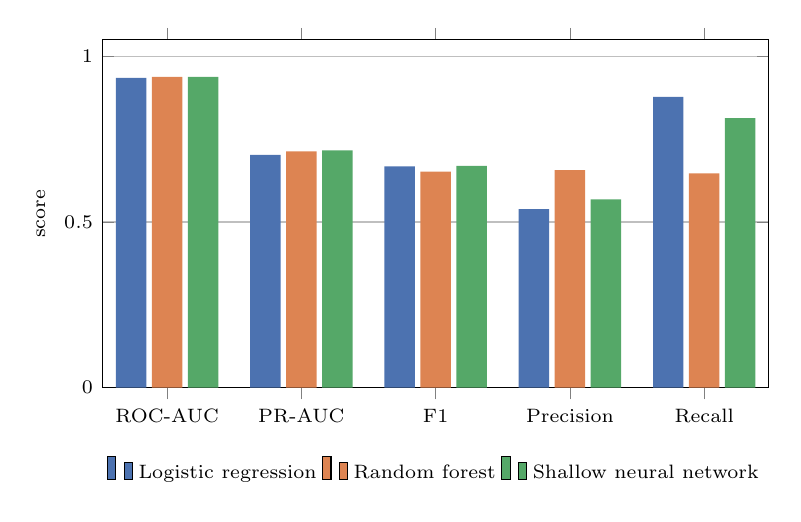
\begin{tikzpicture}
\begin{axis}[ybar, bar width=11pt, width=0.828\linewidth, height=6cm, xtick={0,1,2,3,4}, xticklabels={ROC-AUC,PR-AUC,F1,Precision,Recall}, ymin=0, ymax=1.05, ylabel={score}, ymajorgrids, enlarge x limits=0.12, legend style={at={(0.5,-0.18)}, anchor=north, legend columns=3}]
\addplot[ybar, fill=modelA, draw=none] coordinates {(0,0.935048) (1,0.702575) (2,0.66791) (3,0.539157) (4,0.877451)};
\addplot[ybar, fill=modelB, draw=none] coordinates {(0,0.937628) (1,0.713316) (2,0.651852) (3,0.656716) (4,0.647059)};
\addplot[ybar, fill=modelC, draw=none] coordinates {(0,0.937913) (1,0.716215) (2,0.669355) (3,0.568493) (4,0.813725)};
\legend{Logistic regression, Random forest, Shallow neural network}
\end{axis}
\end{tikzpicture}
\caption{Test-set scores for 2022-2024. ROC-AUC is similar across models. Precision and recall differ because each model uses its own validation cutoff.}
\end{figure}


\begin{table}[H]
\centering
\caption{Scores by model and split. The cutoff maximises F1 on validation and is then frozen for training and test.}
{\footnotesize\rowcolors{2}{white}{zebra}
\begin{tabular}{>{\raggedright\arraybackslash}p{\dimexpr(\linewidth-16\tabcolsep)*244/1000\relax}>{\raggedleft\arraybackslash}p{\dimexpr(\linewidth-16\tabcolsep)*126/1000\relax}>{\raggedleft\arraybackslash}p{\dimexpr(\linewidth-16\tabcolsep)*98/1000\relax}>{\raggedleft\arraybackslash}p{\dimexpr(\linewidth-16\tabcolsep)*114/1000\relax}>{\raggedleft\arraybackslash}p{\dimexpr(\linewidth-16\tabcolsep)*104/1000\relax}>{\raggedleft\arraybackslash}p{\dimexpr(\linewidth-16\tabcolsep)*88/1000\relax}>{\raggedleft\arraybackslash}p{\dimexpr(\linewidth-16\tabcolsep)*121/1000\relax}>{\raggedleft\arraybackslash}p{\dimexpr(\linewidth-16\tabcolsep)*104/1000\relax}}
\toprule
\rowcolor{navy}
\textcolor{white}{\textbf{Model}} & \textcolor{white}{\textbf{Split}} & \textcolor{white}{\textbf{Cutoff}} & \textcolor{white}{\textbf{ROC-AUC}} & \textcolor{white}{\textbf{PR-AUC}} & \textcolor{white}{\textbf{F1}} & \textcolor{white}{\textbf{Precision}} & \textcolor{white}{\textbf{Recall}} \\
\midrule
Logistic regression & train & 0.655 & 0.906 & 0.561 & 0.580 & 0.468 & 0.763 \\
Logistic regression & validation & 0.655 & 0.926 & 0.728 & 0.703 & 0.647 & 0.769 \\
Logistic regression & test & 0.655 & 0.935 & 0.703 & 0.668 & 0.539 & 0.877 \\
Random forest & train & 0.785 & 0.932 & 0.647 & 0.606 & 0.613 & 0.600 \\
Random forest & validation & 0.785 & 0.926 & 0.717 & 0.707 & 0.713 & 0.701 \\
Random forest & test & 0.785 & 0.938 & 0.713 & 0.652 & 0.657 & 0.647 \\
Shallow neural network & train & 0.240 & 0.912 & 0.585 & 0.578 & 0.462 & 0.771 \\
Shallow neural network & validation & 0.240 & 0.928 & 0.738 & 0.713 & 0.677 & 0.752 \\
Shallow neural network & test & 0.240 & 0.938 & 0.716 & 0.669 & 0.568 & 0.814 \\
\bottomrule
\end{tabular}}
\end{table}


On the test set we measure a ROC-AUC of 0.935 for logistic regression, 0.938 for the forest, and 0.938 for the network. Those three numbers are within 0.005 of each other. In the pair reading of ROC-AUC, a true podium finisher outranks a non-podium about 93 to 94 times out of 100. That is a strong ranking. It is also a ranking on which the models do not separate. ROC-AUC compresses the comparison because most rows are not podiums, so a modest number of false alarms barely moves the false-positive rate.


PR-AUC is where they separate. On test, the network scores 0.716, logistic regression 0.703, and the forest 0.713. The test podium rate is 15.0\%, so a useless ranking would sit near 0.150. All three models are far above that floor. The network's lead over logistic regression is 0.014 PR-AUC. We call that a small lead, not a different kind of model. We selected the network before looking at this comparison, because its validation PR-AUC of 0.738 was ahead of 0.728 and 0.717.


The operating points we chose explain the precision and recall bars in Figure 10. At its validation cutoff, logistic regression has test precision 0.539 and recall 0.877. It catches most podiums and accepts more false alarms. The forest has precision 0.657 and recall 0.647. It is the conservative one of the three. The network sits between them, with precision 0.568 and recall 0.814. Test F1 ends up almost tied, from 0.652 to 0.669. Same F1, different mix of missed podiums and false podiums.


The training column is the check for memorizing. All three models have a training PR-AUC below their validation score: 0.561 for logistic regression, 0.647 for the forest, and 0.585 for the network. That was not true of the first forest, which scored 0.919 on training and 0.702 on validation because it had no depth limit and four rows per leaf. The validation search in Section 7.1 limited it. We do not read the higher validation score as the model improving after 2019. Training has a lower podium rate and far more missing qualifying, so the PR-AUC floor on training is lower as well. The comparison we trust is validation against test, where the positive rate is almost the same.


\begin{takeaway}
\textbf{Takeaway.} All three models rank podium finishers well above non-podiums. On the primary score, the network is slightly ahead, but the lead is smaller than the uncertainty of a 39-race validation set (Section 7.2). ROC-AUC hides even that difference.
\end{takeaway}



\subsection{Searching each model's settings, on validation only}


We trained each model on 1950-2019 and scored it on 2020-2021 for every setting in a small grid. Our grid held 8 settings for logistic regression, 9 for the forest, and 12 for the network. We averaged the network over three seeds because its score depends on the initialization. We did not use the test seasons (Table 19).


\begin{table}[H]
\centering
\caption{Search results for the starting settings, the adopted settings, and the top of each grid.}
{\small\rowcolors{2}{white}{zebra}
\begin{tabular}{>{\raggedright\arraybackslash}p{\dimexpr(\linewidth-12\tabcolsep)*206/1000\relax}>{\raggedright\arraybackslash}p{\dimexpr(\linewidth-12\tabcolsep)*324/1000\relax}>{\raggedright\arraybackslash}p{\dimexpr(\linewidth-12\tabcolsep)*147/1000\relax}>{\raggedleft\arraybackslash}p{\dimexpr(\linewidth-12\tabcolsep)*118/1000\relax}>{\raggedleft\arraybackslash}p{\dimexpr(\linewidth-12\tabcolsep)*88/1000\relax}>{\raggedleft\arraybackslash}p{\dimexpr(\linewidth-12\tabcolsep)*118/1000\relax}}
\toprule
\rowcolor{navy}
\textcolor{white}{\textbf{Model}} & \textcolor{white}{\textbf{Setting}} & \textcolor{white}{\textbf{Role}} & \textcolor{white}{\textbf{Val. PR-AUC}} & \textcolor{white}{\textbf{Seed sd}} & \textcolor{white}{\textbf{Train PR-AUC}} \\
\midrule
Logistic regression & C: 10.0, penalty: l2 & best of grid (tie) & 0.7276 & 0.0000 & 0.5610 \\
Logistic regression & C: 1.0, penalty: l2 & starting, kept & 0.7276 & 0.0000 & 0.5610 \\
Random forest & max\_depth: 12, min\_samples\_leaf: 30 & adopted & 0.7174 & 0.0000 & 0.6469 \\
Random forest & max\_depth: None, min\_samples\_leaf: 4 & starting & 0.7021 & 0.0000 & 0.9192 \\
Shallow neural network & hidden\_layer\_sizes: (32, 12), alpha: 0.002 & starting, kept & 0.7248 & 0.0163 & 0.5867 \\
\bottomrule
\end{tabular}}
\end{table}


\textbf{Random forest: improved.} The starting forest ranked 7th of 9. A depth limit of 12 with 30 rows per leaf raises validation PR-AUC from 0.702 to 0.717 and cuts the training score from 0.919 to 0.647, so it no longer memorizes the training seasons. We adopted it, and test PR-AUC rose from 0.689 to 0.713 without the test set taking part in the choice. \textbf{Shallow network: confirmed, not improved.} One layer of 8, 16, 32, or 64 units and two layers of 32 and 12 or 64 and 32, each with two regularization strengths, were all tried. The starting 32 and 12 was best, at 0.7248 over three seeds, so the network is not a deliberately weak choice: smaller ones are worse and larger ones are no better. \textbf{Logistic regression} is insensitive: L1 and L2 penalties and C from 0.01 to 10 all fall between 0.713 and 0.728, and C = 1 with L2 ties for best.



\subsection{How much the validation score can be trusted}


We also asked whether 2019 is a good boundary. The same two models were scored on four validation windows that all end before the test seasons, each training on every earlier season (Table 20). The score depends on the window: logistic regression ranges from 0.689 to 0.728, and the network from 0.668 to 0.738. The window we use is at the top of both ranges, so validation scores are somewhat optimistic.


\begin{table}[H]
\centering
\caption{Validation PR-AUC on four windows that precede the test seasons.}
{\small\rowcolors{2}{white}{zebra}
\begin{tabular}{>{\raggedright\arraybackslash}p{\dimexpr(\linewidth-12\tabcolsep)*219/1000\relax}>{\raggedright\arraybackslash}p{\dimexpr(\linewidth-12\tabcolsep)*156/1000\relax}>{\raggedleft\arraybackslash}p{\dimexpr(\linewidth-12\tabcolsep)*141/1000\relax}>{\raggedleft\arraybackslash}p{\dimexpr(\linewidth-12\tabcolsep)*141/1000\relax}>{\raggedleft\arraybackslash}p{\dimexpr(\linewidth-12\tabcolsep)*188/1000\relax}>{\raggedleft\arraybackslash}p{\dimexpr(\linewidth-12\tabcolsep)*156/1000\relax}}
\toprule
\rowcolor{navy}
\textcolor{white}{\textbf{Validation window}} & \textcolor{white}{\textbf{Train years}} & \textcolor{white}{\textbf{Train rows}} & \textcolor{white}{\textbf{Val. races}} & \textcolor{white}{\textbf{LogReg PR-AUC}} & \textcolor{white}{\textbf{MLP PR-AUC}} \\
\midrule
2014-2015 & 1950-2013 & 22,042 & 38 & 0.7208 & 0.7137 \\
2016-2017 & 1950-2015 & 22,827 & 41 & 0.7278 & 0.6683 \\
2018-2019 & 1950-2017 & 23,689 & 42 & 0.6891 & 0.6982 \\
2020-2021 (used) & 1950-2019 & 24,529 & 39 & 0.7276 & 0.7385 \\
\bottomrule
\end{tabular}}
\end{table}


To measure the uncertainty directly we resampled whole validation races (Table 21). With 39 races, each model's PR-AUC has a 95\% interval about 0.2 wide. The difference between the network and logistic regression is +0.011 with an interval from $-$0.010 to +0.031, and the forest's difference also includes zero. The data therefore do not show that any model beats the baseline, and we report the ranking as a tie within validation uncertainty. The chronological split stays because it is the only one with no same-race and no future leakage.


\begin{table}[H]
\centering
\caption{Bootstrap over the 39 validation races. The last two rows are differences from logistic regression.}
{\small\rowcolors{2}{white}{zebra}
\begin{tabular}{>{\raggedright\arraybackslash}p{\dimexpr(\linewidth-8\tabcolsep)*484/1000\relax}>{\raggedleft\arraybackslash}p{\dimexpr(\linewidth-8\tabcolsep)*203/1000\relax}>{\raggedleft\arraybackslash}p{\dimexpr(\linewidth-8\tabcolsep)*156/1000\relax}>{\raggedleft\arraybackslash}p{\dimexpr(\linewidth-8\tabcolsep)*156/1000\relax}}
\toprule
\rowcolor{navy}
\textcolor{white}{\textbf{Comparison}} & \textcolor{white}{\textbf{Validation PR-AUC}} & \textcolor{white}{\textbf{95\% low}} & \textcolor{white}{\textbf{95\% high}} \\
\midrule
Logistic regression & 0.7276 & 0.6167 & 0.8364 \\
Random forest & 0.7174 & 0.6028 & 0.8338 \\
Shallow neural network & 0.7385 & 0.6270 & 0.8450 \\
Random forest minus Logistic regression & $-$0.0102 & $-$0.0441 & 0.0276 \\
Shallow neural network minus Logistic regression & 0.0109 & $-$0.0105 & 0.0307 \\
\bottomrule
\end{tabular}}
\end{table}



\section{Removing the grid hurts more than removing anything else}


In our ablation we retrain logistic regression after deleting one feature group, then record the change in validation PR-AUC. We want to see which group the linear model was using, on the same rows as Section 7. Figure 11 shows the change from the full model. A bar to the left of zero is a loss.


\begin{figure}[H]
\centering
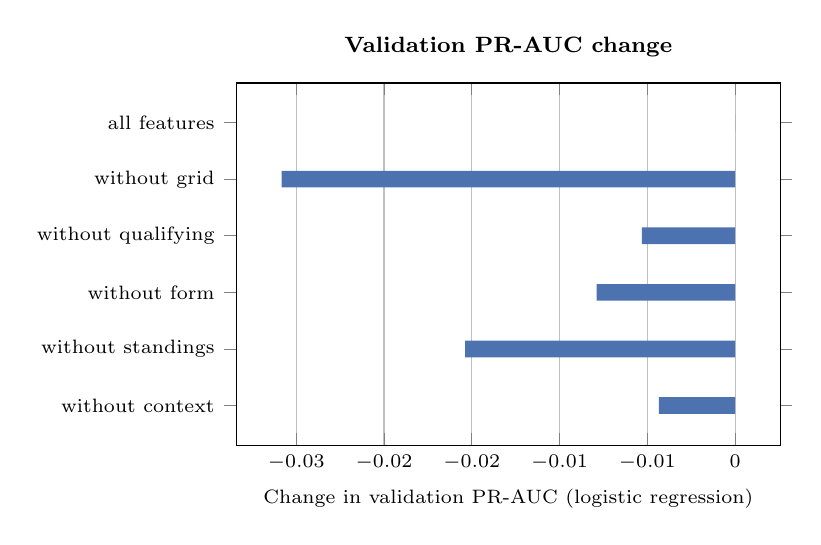
\begin{tikzpicture}
\begin{axis}[xbar, bar width=6pt, width=0.570\linewidth, height=4.6cm, scale only axis, ytick={0,1,2,3,4,5}, yticklabels={all features,without grid,without qualifying,without form,without standings,without context}, y dir=reverse, ymin=-0.7, ymax=5.7, xlabel={Change in validation PR-AUC (logistic regression)}, xmajorgrids, yticklabel style={font=\scriptsize}, enlarge x limits=0.1, title={Validation PR-AUC change}, ]
\addplot[xbar, fill=modelA, draw=none] coordinates {(0,0) (-0.0258366,1) (-0.00530358,2) (-0.00788891,3) (-0.0153724,4) (-0.00434181,5)};
\end{axis}
\end{tikzpicture}
\caption{Change in validation PR-AUC when one feature group is removed from logistic regression. Zero is the full 17-feature model.}
\end{figure}


\begin{table}[H]
\centering
\caption{Ablation of logistic regression on the 2020-2021 validation seasons.}
{\small\rowcolors{2}{white}{zebra}
\begin{tabular}{>{\raggedright\arraybackslash}p{\dimexpr(\linewidth-10\tabcolsep)*291/1000\relax}>{\raggedleft\arraybackslash}p{\dimexpr(\linewidth-10\tabcolsep)*197/1000\relax}>{\raggedleft\arraybackslash}p{\dimexpr(\linewidth-10\tabcolsep)*154/1000\relax}>{\raggedleft\arraybackslash}p{\dimexpr(\linewidth-10\tabcolsep)*154/1000\relax}>{\raggedleft\arraybackslash}p{\dimexpr(\linewidth-10\tabcolsep)*205/1000\relax}}
\toprule
\rowcolor{navy}
\textcolor{white}{\textbf{Variant}} & \textcolor{white}{\textbf{Features kept}} & \textcolor{white}{\textbf{PR-AUC}} & \textcolor{white}{\textbf{ROC-AUC}} & \textcolor{white}{\textbf{PR-AUC change}} \\
\midrule
all features & 17 & 0.728 & 0.926 & +0.000 \\
without grid & 13 & 0.702 & 0.921 & $-$0.026 \\
without qualifying & 14 & 0.722 & 0.924 & $-$0.005 \\
without form & 14 & 0.720 & 0.923 & $-$0.008 \\
without standings & 13 & 0.712 & 0.924 & $-$0.015 \\
without context & 14 & 0.723 & 0.925 & $-$0.004 \\
\bottomrule
\end{tabular}}
\end{table}


The full model sits at 0.728. Dropping the grid group costs 0.026 PR-AUC, the largest loss. Standings are next, at 0.015. Form, qualifying, and context cost 0.008, 0.005, and 0.004. The qualifying drop is small once the grid is already in the model. That fits the sport and the earlier definition: the published grid already contains qualifying order, plus any penalty. We do not conclude that qualifying is irrelevant on its own. We conclude that, next to the grid, it is mostly repeated information.


ROC-AUC barely notices the same deletion. It moves from 0.926 to 0.921 when the grid group is removed. This is the same lesson as the model comparison we drew in Section 7. A metric that stays high while the primary score drops is a poor guide for what to keep.


The context and qualifying changes are about the same size as the logistic-regression preprocessing gaps in Section 6. On 39 validation races, we treat those as small. The grid drop is several times larger, and it agrees with the descriptive ladder in Section 4.2, where podium rate falls from about 55\% at the front of the grid to under 1\% at the back.


\begin{takeaway}
\textbf{Takeaway.} For the linear model, the final grid is the group we cannot remove without a visible loss. Recent standings help. Qualifying, form, and calendar context add less once the grid is present.
\end{takeaway}



\section{What the forest relies on, and where the two explanations differ}


The explanations in this section are for the random forest, not for the neural network we selected in Section 7. Tree explanations apply directly to the forest. We do not borrow them as an account of the network. Permutation importance shuffles one validation column at a time and measures the drop in PR-AUC. Global SHAP averages the size of each feature's push across 400 validation rows. Local SHAP is one of those rows. A positive value pushes that row toward a podium relative to the forest's background. A negative value pushes it away. These are associations inside the fitted forest. They are not estimates of what would happen if we moved a driver up the grid.



\subsection{Permutation importance}


\begin{figure}[H]
\centering
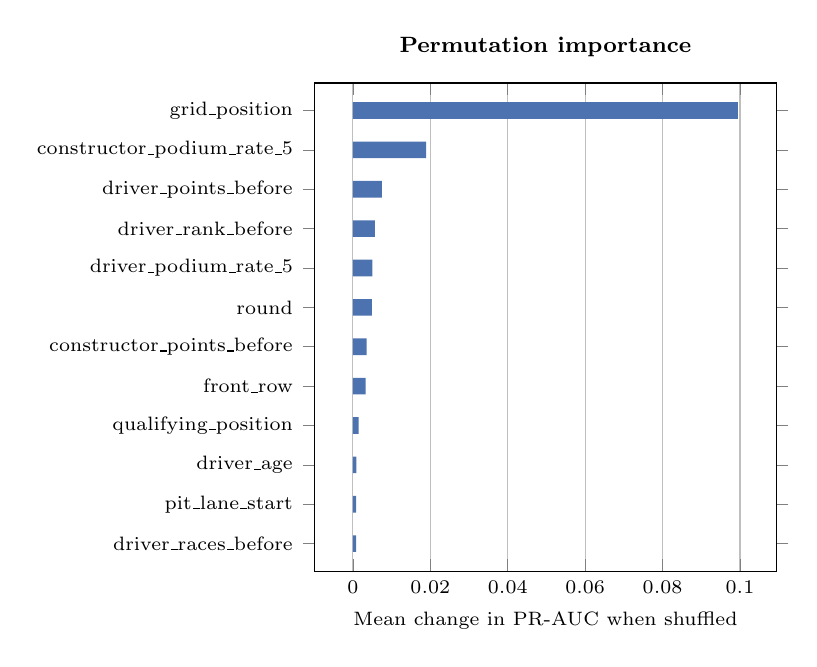
\begin{tikzpicture}
\begin{axis}[xbar, bar width=6pt, width=0.484\linewidth, height=6.2cm, scale only axis, ytick={0,1,2,3,4,5,6,7,8,9,10,11}, yticklabels={grid\_position,constructor\_podium\_rate\_5,driver\_points\_before,driver\_rank\_before,driver\_podium\_rate\_5,round,constructor\_points\_before,front\_row,qualifying\_position,driver\_age,pit\_lane\_start,driver\_races\_before}, y dir=reverse, ymin=-0.7, ymax=11.7, xlabel={Mean change in PR-AUC when shuffled}, xmajorgrids, xmin=0, yticklabel style={font=\scriptsize}, enlarge x limits=0.1, title={Permutation importance}, ]
\addplot[xbar, fill=modelA, draw=none] coordinates {(0.099476,0) (0.0188843,1) (0.00748939,2) (0.00567179,3) (0.00500172,4) (0.00488749,5) (0.0035371,6) (0.00329779,7) (0.00146695,8) (0.000866121,9) (0.000812563,10) (0.000807814,11)};
\end{axis}
\end{tikzpicture}
\caption{Permutation importance on a validation sample, scored with PR-AUC. A taller bar means shuffling that column hurt the forest more.}
\end{figure}


\begin{table}[H]
\centering
\caption{Largest positive permutation importances, followed by the three most negative. Computed on the random forest and a validation sample.}
{\small\rowcolors{2}{white}{zebra}
\begin{tabular}{>{\raggedright\arraybackslash}p{\dimexpr(\linewidth-4\tabcolsep)*533/1000\relax}>{\raggedleft\arraybackslash}p{\dimexpr(\linewidth-4\tabcolsep)*467/1000\relax}}
\toprule
\rowcolor{navy}
\textcolor{white}{\textbf{Feature}} & \textcolor{white}{\textbf{Mean PR-AUC change when shuffled}} \\
\midrule
grid\_position & +0.099 \\
constructor\_podium\_rate\_5 & +0.019 \\
driver\_points\_before & +0.007 \\
driver\_rank\_before & +0.006 \\
driver\_podium\_rate\_5 & +0.005 \\
round & +0.005 \\
constructor\_points\_before & +0.004 \\
front\_row & +0.003 \\
qualifying\_time\_seconds & $-$0.004 \\
constructor\_rank\_before & $-$0.002 \\
qualifying\_missing & +0.000 \\
\bottomrule
\end{tabular}}
\end{table}


Grid position is in a class of its own, at +0.099. The next feature, constructor\_podium\_rate\_5, is +0.019, about 19\% of that, and every other feature is +0.007 or smaller. Driver podium rate is ranked 5 at +0.005, and year sits at +0.000. Shuffling qualifying\_time\_seconds changes PR-AUC by $-$0.004: the score rises slightly when the column is destroyed. We read a negative value as the forest not getting stable help from that column on these rows. We do not read it as evidence that the feature causes worse finishes.



\subsection{Global and local SHAP}


Figure 13 asks the same question with SHAP. Each validation prediction is split into one credit per feature, and we average the size of those credits. The sign is not in this chart. A tall bar means the forest moved the prediction a long way when that feature changed, whether the move was toward a podium or away from one.


\begin{figure}[H]
\centering
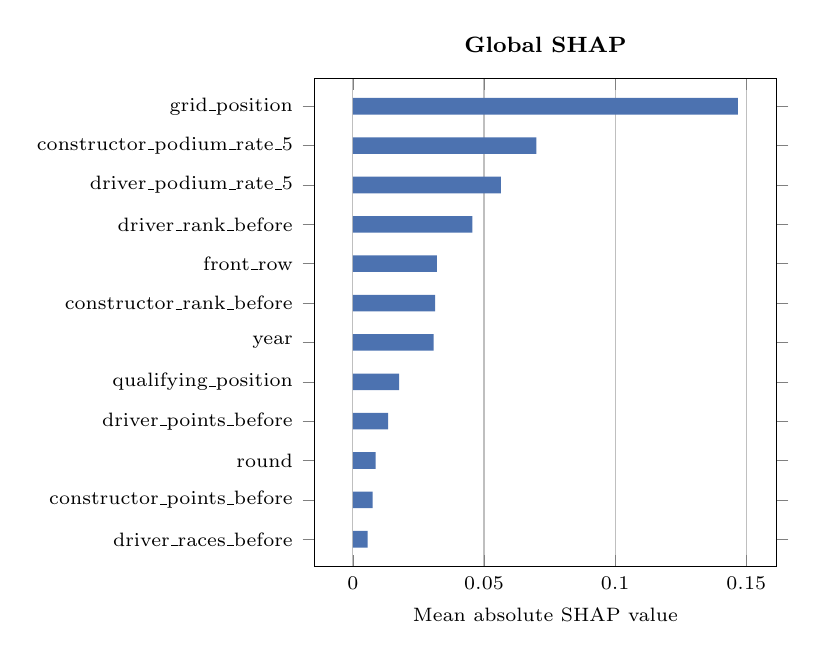
\begin{tikzpicture}
\begin{axis}[xbar, bar width=6pt, width=0.484\linewidth, height=6.2cm, scale only axis, ytick={0,1,2,3,4,5,6,7,8,9,10,11}, yticklabels={grid\_position,constructor\_podium\_rate\_5,driver\_podium\_rate\_5,driver\_rank\_before,front\_row,constructor\_rank\_before,year,qualifying\_position,driver\_points\_before,round,constructor\_points\_before,driver\_races\_before}, y dir=reverse, ymin=-0.7, ymax=11.7, xlabel={Mean absolute SHAP value}, xmajorgrids, xmin=0, yticklabel style={font=\scriptsize}, enlarge x limits=0.1, title={Global SHAP}, ]
\addplot[xbar, fill=modelA, draw=none] coordinates {(0.146834,0) (0.0699154,1) (0.0564363,2) (0.0455589,3) (0.0319986,4) (0.0313301,5) (0.0307951,6) (0.0175809,7) (0.013431,8) (0.00867357,9) (0.00753165,10) (0.00561299,11)};
\end{axis}
\end{tikzpicture}
\caption{Mean absolute SHAP value by feature for the random forest, over 400 validation rows. This measures how large a feature's push is, not whether the push is positive.}
\end{figure}


\begin{table}[H]
\centering
\caption{Eight largest mean absolute SHAP values for the random forest on the validation sample.}
{\small\rowcolors{2}{white}{zebra}
\begin{tabular}{>{\raggedright\arraybackslash}p{\dimexpr(\linewidth-4\tabcolsep)*567/1000\relax}>{\raggedleft\arraybackslash}p{\dimexpr(\linewidth-4\tabcolsep)*433/1000\relax}}
\toprule
\rowcolor{navy}
\textcolor{white}{\textbf{Feature}} & \textcolor{white}{\textbf{Mean absolute SHAP}} \\
\midrule
grid\_position & 0.147 \\
constructor\_podium\_rate\_5 & 0.070 \\
driver\_podium\_rate\_5 & 0.056 \\
driver\_rank\_before & 0.046 \\
front\_row & 0.032 \\
constructor\_rank\_before & 0.031 \\
year & 0.031 \\
qualifying\_position & 0.018 \\
\bottomrule
\end{tabular}}
\end{table}


Global SHAP also puts grid position first, at 0.147, and constructor podium rate second (0.070), the same top two as permutation importance. Driver podium rate follows at 0.056. The two methods differ below that. Year has a mean SHAP value of 0.031 (rank 7) but a permutation importance of +0.000, and driver points before the race is the reverse: rank 3 under permutation and rank 9 under SHAP. A reasonable reading is that year, form, and the standings overlap with each other and with the grid. The trees use them, but once the other columns are left intact, destroying one of them alone does not collapse the score. We treat the shared finding as the reliable one: grid position first, constructor form second.


Figure 14 is one validation row from that sample, not a row we picked because it looks tidy. It is George Russell, Williams, 2021 Dutch Grand Prix. He qualified and started 11th in a field of 20, sat 15th in the championship, and had a podium in one of his previous five starts (driver podium rate 0.2). He did not podium.


\begin{figure}[H]
\centering
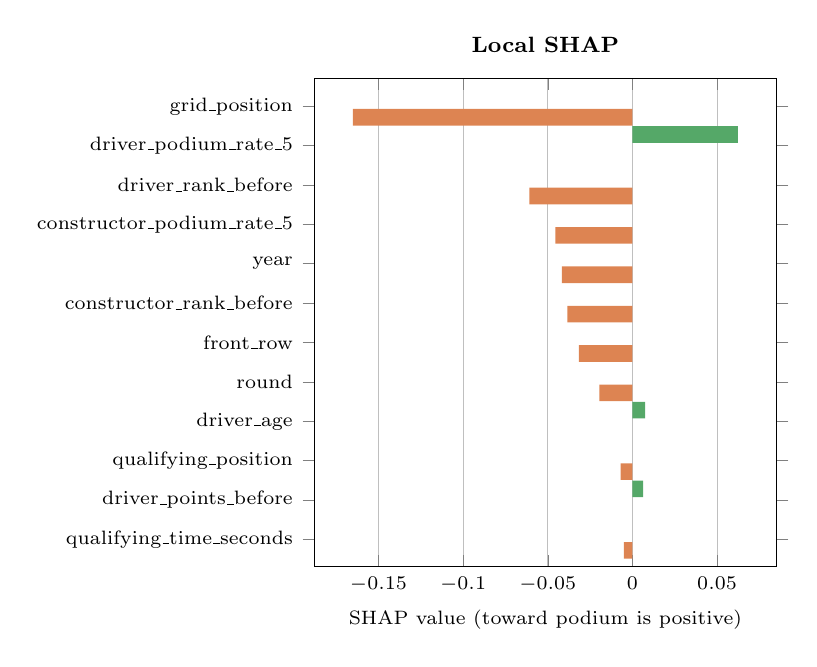
\begin{tikzpicture}
\begin{axis}[xbar, bar width=6pt, width=0.484\linewidth, height=6.2cm, scale only axis, ytick={0,1,2,3,4,5,6,7,8,9,10,11}, yticklabels={grid\_position,driver\_podium\_rate\_5,driver\_rank\_before,constructor\_podium\_rate\_5,year,constructor\_rank\_before,front\_row,round,driver\_age,qualifying\_position,driver\_points\_before,qualifying\_time\_seconds}, y dir=reverse, ymin=-0.7, ymax=11.7, xlabel={SHAP value (toward podium is positive)}, xmajorgrids, yticklabel style={font=\scriptsize}, enlarge x limits=0.1, title={Local SHAP}, ]
\addplot[xbar, fill=modelB, draw=none] coordinates {(-0.165099,0) (-0.0608252,2) (-0.045578,3) (-0.0417418,4) (-0.0383849,5) (-0.0316522,6) (-0.0195359,7) (-0.00699777,9) (-0.00507363,11)};
\addplot[xbar, fill=modelC, draw=none] coordinates {(0.0623457,1) (0.00743139,8) (0.00626201,10)};
\end{axis}
\end{tikzpicture}
\caption{SHAP contributions for one validation row: Russell, Williams, 2021 Dutch Grand Prix, started 11th and did not podium. Negative values push the forest away from a podium.}
\end{figure}


\begin{table}[H]
\centering
\caption{Largest SHAP contributions for the Russell validation row. The sign is the direction of the push.}
{\small\rowcolors{2}{white}{zebra}
\begin{tabular}{>{\raggedright\arraybackslash}p{\dimexpr(\linewidth-6\tabcolsep)*500/1000\relax}>{\raggedleft\arraybackslash}p{\dimexpr(\linewidth-6\tabcolsep)*232/1000\relax}>{\raggedleft\arraybackslash}p{\dimexpr(\linewidth-6\tabcolsep)*268/1000\relax}}
\toprule
\rowcolor{navy}
\textcolor{white}{\textbf{Feature}} & \textcolor{white}{\textbf{SHAP value}} & \textcolor{white}{\textbf{Observed value}} \\
\midrule
grid\_position & $-$0.165 & 11.0 \\
driver\_podium\_rate\_5 & +0.062 & 0.2 \\
driver\_rank\_before & $-$0.061 & 15.0 \\
constructor\_podium\_rate\_5 & $-$0.046 & 0.1 \\
year & $-$0.042 & 2021.0 \\
constructor\_rank\_before & $-$0.038 & 8.0 \\
\bottomrule
\end{tabular}}
\end{table}


The largest push is grid\_position = 11, and it is negative ($-$0.165). The next negative push is driver\_rank\_before = 15 ($-$0.061). The clearest positive push is driver\_podium\_rate\_5 = 0.2 (+0.062), and it is smaller than the grid push. We observe a row where recent form points up and the start position points down, with the start position winning inside this forest. That is one example. It matches the ablation, and it matches the grid ladder in Section 4, but a single row is not a general law.



\subsection{Local LIME explanation}


LIME provides the required model-agnostic local explanation for the same fixed validation case. We create 5,000 nearby records by either retaining each observed feature or replacing it with a value drawn from the training seasons. The random forest scores those records, and a distance-weighted ridge model approximates the forest around the explained row. A positive coefficient pushes the local surrogate toward a podium; a negative coefficient pushes it away.


\begin{figure}[H]
\centering
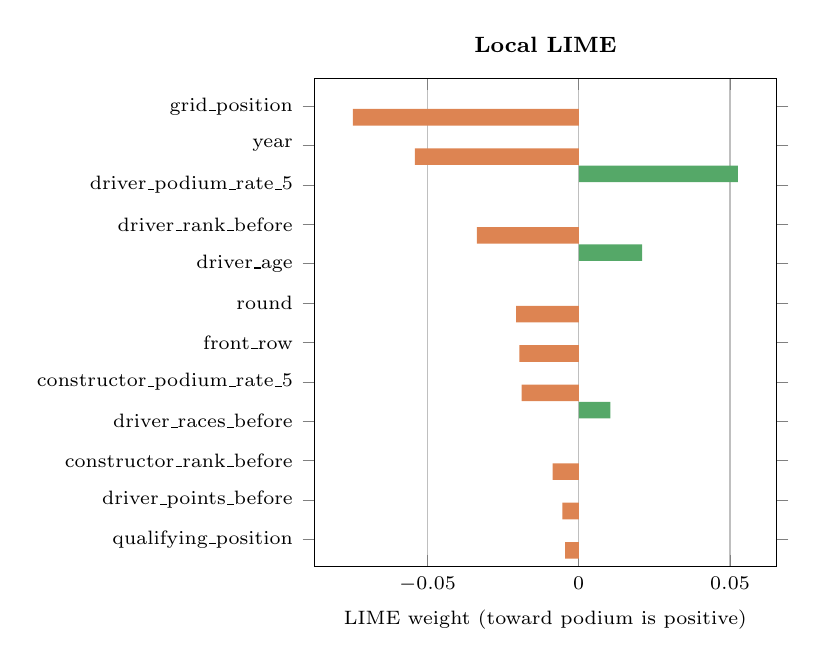
\begin{tikzpicture}
\begin{axis}[xbar, bar width=6pt, width=0.484\linewidth, height=6.2cm, scale only axis, ytick={0,1,2,3,4,5,6,7,8,9,10,11}, yticklabels={grid\_position,year,driver\_podium\_rate\_5,driver\_rank\_before,driver\_age,round,front\_row,constructor\_podium\_rate\_5,driver\_races\_before,constructor\_rank\_before,driver\_points\_before,qualifying\_position}, y dir=reverse, ymin=-0.7, ymax=11.7, xlabel={LIME weight (toward podium is positive)}, xmajorgrids, yticklabel style={font=\scriptsize}, enlarge x limits=0.1, title={Local LIME}, ]
\addplot[xbar, fill=modelB, draw=none] coordinates {(-0.0746564,0) (-0.0541669,1) (-0.0336603,3) (-0.0207338,5) (-0.0196676,6) (-0.0188447,7) (-0.00865997,9) (-0.00540089,10) (-0.00447633,11)};
\addplot[xbar, fill=modelC, draw=none] coordinates {(0.0526331,2) (0.020962,4) (0.0104363,8)};
\end{axis}
\end{tikzpicture}
\caption{Local LIME contributions for one fixed validation prediction. The black-box probability is 0.161, the local surrogate estimate is 0.157, and weighted local R-squared is 0.206.}
\end{figure}


\begin{table}[H]
\centering
\caption{Largest absolute LIME weights for the fixed validation row.}
{\small\rowcolors{2}{white}{zebra}
\begin{tabular}{>{\raggedright\arraybackslash}p{\dimexpr(\linewidth-6\tabcolsep)*500/1000\relax}>{\raggedleft\arraybackslash}p{\dimexpr(\linewidth-6\tabcolsep)*232/1000\relax}>{\raggedleft\arraybackslash}p{\dimexpr(\linewidth-6\tabcolsep)*268/1000\relax}}
\toprule
\rowcolor{navy}
\textcolor{white}{\textbf{Feature}} & \textcolor{white}{\textbf{LIME weight}} & \textcolor{white}{\textbf{Observed value}} \\
\midrule
grid\_position & $-$0.075 & 11.0 \\
year & $-$0.054 & 2021.0 \\
driver\_podium\_rate\_5 & +0.053 & 0.2 \\
driver\_rank\_before & $-$0.034 & 15.0 \\
driver\_age & +0.021 & 23.6 \\
round & $-$0.021 & 13.0 \\
front\_row & $-$0.020 & 0.0 \\
constructor\_podium\_rate\_5 & $-$0.019 & 0.1 \\
\bottomrule
\end{tabular}}
\end{table}


The weighted local R-squared is 0.206. This fidelity value tells us how closely the simple surrogate follows the forest in the sampled neighborhood, so we read the local coefficients together with it rather than as global effects.


\begin{takeaway}
\textbf{Takeaway.} Grid position is the feature the explanation methods agree on, with constructor form second under both. They differ on the smaller features, such as year and driver points, which is what we expect when form, standings, and year overlap with the grid. None of these values is a causal effect of starting further forward.
\end{takeaway}



\section{Two predictions from the selected network}


The examples use the shallow neural network, because it had the best validation PR-AUC. Its frozen cutoff is 0.240. Missing inputs are filled by the imputer that was fit on the training years. We show one complete historical row and one partial record that was never a real entry.


The complete row is Lewis Hamilton, Mercedes, 2022 Saudi Arabian Grand Prix, round 2. He qualified 16th and started 15th in a field of 20. His previous five starts in this table were all podiums (driver rate 1.0), the constructor's recent podium rate was 0.7, he was third in the championship on 15 points, and Mercedes was second on 27 points. The network gives this row a podium probability of 0.087. That is below 0.240, so the predicted label is not a podium. The actual result was not a podium. Strong recent form and a high championship position did not overcome 15th on the grid, either in the race or in the model.


The partial record supplies only what we chose to type in: grid position 3, not a pit-lane start, not a front-row start, a field of 20, season 2024, round 5. Every other feature is missing and is replaced with the training median. The network returns 0.032, also below the cutoff, so the predicted label is again not a podium. This record has no true result, because it is not a driver who started a race.


We should not read 0.032 as the historical podium rate of cars that start third. Section 4.2 puts that rate near 55\% for grid positions 1-3. The partial row is a third-place start glued onto a median historical driver, and the median driver in a 1950-2019 training set is not a podium contender. The low probability is what this imputer does with a half-empty row. It is evidence that the function accepts missing fields. It is not evidence about the front of the grid.


\begin{takeaway}
\textbf{Takeaway.} On a real 2022 row, the selected model correctly stayed below its cutoff for a 15th-place start despite a perfect recent podium run. On a synthetic partial row, the number is an imputed profile, and we do not interpret it as a base rate.
\end{takeaway}



\section{What we do not want the results to be taken to say}


Qualifying coverage is a property of this snapshot. We described it, and we kept a missingness flag, but we cannot tell from the chart alone how much of the pre-1994 gap is history and how much is the way the public tables were filled.


Constructor identifiers reset when a team is renamed, so form and standings for the new name start again. We left it that way on purpose, which means a works team that changes its entry name looks like a new constructor to us.


The home analysis depends on a nationality-to-country map. Drivers we could not map are excluded, and drivers with more than one sporting nationality are forced into one label. The small home samples in the front of the grid mean a one-point gap is not something we would defend as a precise estimate.


The mechanical list is a rule we wrote down, not a measurement from the car. Ambiguous statuses can fall outside it. Leading rates such as Caterham's rest on a few dozen starts. The lower 2022-2024 totals are consistent with a more reliable field, and they are also consistent with changes in how retirements were described.


Validation is 39 races. We used it to pick a cutoff and a model, which is what a held-out test set requires, and we do not pretend it can rank effects of a few thousandths. A bootstrap over those races gives each PR-AUC an interval about 0.2 wide, and the differences between the models fall inside it. Regulation changes in 2014 and 2022 sit inside the eras we compared. The models are associating historical patterns. They do not tell a team what would happen if it started one place further forward, and a probability is not a guarantee about the next race.



\section{What the evidence supports}


The tables join, and after 85 shared-drive groups are resolved we have one row per driver per race, 26,668 of them, with a podium rate of 12.7\%. Qualifying is missing for most of the early history and nearly complete from 2003, so the grid is the starting-order feature we can actually follow from 1950.


Descriptively, front-row cars podium far more often than the field, and more often again after 2013. Home nationality, inside a grid band, does not produce a consistent extra podium rate. Mechanical retirement rates, on our component list and among teams with at least 20 starts, are lower in 2022-2024 than in 2014-2021, and the highest rates belong to shorter entries.


Predictively, logistic regression, a random forest, and a shallow network all clear the PR-AUC baseline of the recent seasons by a wide margin. The network is the one we select from the validation scores, and the untouched test seasons still place it slightly first, although the three models are within validation uncertainty of each other. Ablation, permutation, and SHAP agree that grid position carries the prediction, and permutation and SHAP also agree that constructor form comes second. They differ on the smaller features, and we do not force them to agree. The Hamilton example is the same story in one row: a recent run of podiums, from 15th on the grid, was not enough.

\end{document}
